% Options for packages loaded elsewhere
\PassOptionsToPackage{unicode}{hyperref}
\PassOptionsToPackage{hyphens}{url}
%
\documentclass[
]{article}
\usepackage{amsmath,amssymb}
\usepackage{iftex}
\ifPDFTeX
  \usepackage[T1]{fontenc}
  \usepackage[utf8]{inputenc}
  \usepackage{textcomp} % provide euro and other symbols
\else % if luatex or xetex
  \usepackage{unicode-math} % this also loads fontspec
  \defaultfontfeatures{Scale=MatchLowercase}
  \defaultfontfeatures[\rmfamily]{Ligatures=TeX,Scale=1}
\fi
\usepackage{lmodern}
\ifPDFTeX\else
  % xetex/luatex font selection
\fi
% Use upquote if available, for straight quotes in verbatim environments
\IfFileExists{upquote.sty}{\usepackage{upquote}}{}
\IfFileExists{microtype.sty}{% use microtype if available
  \usepackage[]{microtype}
  \UseMicrotypeSet[protrusion]{basicmath} % disable protrusion for tt fonts
}{}
\makeatletter
\@ifundefined{KOMAClassName}{% if non-KOMA class
  \IfFileExists{parskip.sty}{%
    \usepackage{parskip}
  }{% else
    \setlength{\parindent}{0pt}
    \setlength{\parskip}{6pt plus 2pt minus 1pt}}
}{% if KOMA class
  \KOMAoptions{parskip=half}}
\makeatother
\usepackage{xcolor}
\usepackage[margin=1in]{geometry}
\usepackage{color}
\usepackage{fancyvrb}
\newcommand{\VerbBar}{|}
\newcommand{\VERB}{\Verb[commandchars=\\\{\}]}
\DefineVerbatimEnvironment{Highlighting}{Verbatim}{commandchars=\\\{\}}
% Add ',fontsize=\small' for more characters per line
\usepackage{framed}
\definecolor{shadecolor}{RGB}{248,248,248}
\newenvironment{Shaded}{\begin{snugshade}}{\end{snugshade}}
\newcommand{\AlertTok}[1]{\textcolor[rgb]{0.94,0.16,0.16}{#1}}
\newcommand{\AnnotationTok}[1]{\textcolor[rgb]{0.56,0.35,0.01}{\textbf{\textit{#1}}}}
\newcommand{\AttributeTok}[1]{\textcolor[rgb]{0.13,0.29,0.53}{#1}}
\newcommand{\BaseNTok}[1]{\textcolor[rgb]{0.00,0.00,0.81}{#1}}
\newcommand{\BuiltInTok}[1]{#1}
\newcommand{\CharTok}[1]{\textcolor[rgb]{0.31,0.60,0.02}{#1}}
\newcommand{\CommentTok}[1]{\textcolor[rgb]{0.56,0.35,0.01}{\textit{#1}}}
\newcommand{\CommentVarTok}[1]{\textcolor[rgb]{0.56,0.35,0.01}{\textbf{\textit{#1}}}}
\newcommand{\ConstantTok}[1]{\textcolor[rgb]{0.56,0.35,0.01}{#1}}
\newcommand{\ControlFlowTok}[1]{\textcolor[rgb]{0.13,0.29,0.53}{\textbf{#1}}}
\newcommand{\DataTypeTok}[1]{\textcolor[rgb]{0.13,0.29,0.53}{#1}}
\newcommand{\DecValTok}[1]{\textcolor[rgb]{0.00,0.00,0.81}{#1}}
\newcommand{\DocumentationTok}[1]{\textcolor[rgb]{0.56,0.35,0.01}{\textbf{\textit{#1}}}}
\newcommand{\ErrorTok}[1]{\textcolor[rgb]{0.64,0.00,0.00}{\textbf{#1}}}
\newcommand{\ExtensionTok}[1]{#1}
\newcommand{\FloatTok}[1]{\textcolor[rgb]{0.00,0.00,0.81}{#1}}
\newcommand{\FunctionTok}[1]{\textcolor[rgb]{0.13,0.29,0.53}{\textbf{#1}}}
\newcommand{\ImportTok}[1]{#1}
\newcommand{\InformationTok}[1]{\textcolor[rgb]{0.56,0.35,0.01}{\textbf{\textit{#1}}}}
\newcommand{\KeywordTok}[1]{\textcolor[rgb]{0.13,0.29,0.53}{\textbf{#1}}}
\newcommand{\NormalTok}[1]{#1}
\newcommand{\OperatorTok}[1]{\textcolor[rgb]{0.81,0.36,0.00}{\textbf{#1}}}
\newcommand{\OtherTok}[1]{\textcolor[rgb]{0.56,0.35,0.01}{#1}}
\newcommand{\PreprocessorTok}[1]{\textcolor[rgb]{0.56,0.35,0.01}{\textit{#1}}}
\newcommand{\RegionMarkerTok}[1]{#1}
\newcommand{\SpecialCharTok}[1]{\textcolor[rgb]{0.81,0.36,0.00}{\textbf{#1}}}
\newcommand{\SpecialStringTok}[1]{\textcolor[rgb]{0.31,0.60,0.02}{#1}}
\newcommand{\StringTok}[1]{\textcolor[rgb]{0.31,0.60,0.02}{#1}}
\newcommand{\VariableTok}[1]{\textcolor[rgb]{0.00,0.00,0.00}{#1}}
\newcommand{\VerbatimStringTok}[1]{\textcolor[rgb]{0.31,0.60,0.02}{#1}}
\newcommand{\WarningTok}[1]{\textcolor[rgb]{0.56,0.35,0.01}{\textbf{\textit{#1}}}}
\usepackage{graphicx}
\makeatletter
\def\maxwidth{\ifdim\Gin@nat@width>\linewidth\linewidth\else\Gin@nat@width\fi}
\def\maxheight{\ifdim\Gin@nat@height>\textheight\textheight\else\Gin@nat@height\fi}
\makeatother
% Scale images if necessary, so that they will not overflow the page
% margins by default, and it is still possible to overwrite the defaults
% using explicit options in \includegraphics[width, height, ...]{}
\setkeys{Gin}{width=\maxwidth,height=\maxheight,keepaspectratio}
% Set default figure placement to htbp
\makeatletter
\def\fps@figure{htbp}
\makeatother
\setlength{\emergencystretch}{3em} % prevent overfull lines
\providecommand{\tightlist}{%
  \setlength{\itemsep}{0pt}\setlength{\parskip}{0pt}}
\setcounter{secnumdepth}{-\maxdimen} % remove section numbering
\ifLuaTeX
  \usepackage{selnolig}  % disable illegal ligatures
\fi
\usepackage{bookmark}
\IfFileExists{xurl.sty}{\usepackage{xurl}}{} % add URL line breaks if available
\urlstyle{same}
\hypersetup{
  pdftitle={CACCS: Secuencia de taller de RStudio -- Parte 2},
  pdfauthor={Rashid C.J. Marcano Rivera},
  hidelinks,
  pdfcreator={LaTeX via pandoc}}

\title{CACCS: Secuencia de taller de RStudio -- Parte 2}
\author{Rashid C.J. Marcano Rivera}
\date{11 de oct.ᵉ de 2024}

\begin{document}
\maketitle

{
\setcounter{tocdepth}{2}
\tableofcontents
}
\textbf{Visualización de datos}

Este taller está basado en viñetas de RStudio con tidyverse (en
específico \href{https://ggplot2.tidyverse.org}{\texttt{ggplot},}) así
como elementos y ejemplos del libro de Rafael Irizarry
\href{https://leanpub.com/dslibro}{disponible aquí} o de manera similar
a los html producidos en este taller y y más actualizada
\href{https://rafalab.dfci.harvard.edu/dslibro/}{aquí}. Finalmente la
parte del censo proviene en parte de código ajustado del libro
\href{https://urbanspatial.github.io/PublicPolicyAnalytics/introduction.html}{Public
Policy Analytics: Code \& Context for Data Science in Government}, por
Ken Steif.

\emph{Si aún no has instalado R, está
\href{http://cran.us.r-project.org/}{aquí}. Acto seguido,
\href{https://posit.co/download/rstudio-desktop/}{baja RStudio}. Puedes
también ir a la nube \href{https://posit.cloud/}{en Posit Cloud}.}

\section{Visualización de datos:
porqués}\label{visualizaciuxf3n-de-datos-porquuxe9s}

Ver números y cadenas de caracteres que forman un conjunto de datos
puede ser interesante, o no, pero normalmente no tiene tanta utilidad.
Por ejemplo

\begin{Shaded}
\begin{Highlighting}[]
\FunctionTok{library}\NormalTok{(wooldridge)}

\FunctionTok{data}\NormalTok{(wage1)}
\FunctionTok{head}\NormalTok{(wage1)}
\end{Highlighting}
\end{Shaded}

\begin{verbatim}
##   wage educ exper tenure nonwhite female married numdep smsa northcen south
## 1 3.10   11     2      0        0      1       0      2    1        0     0
## 2 3.24   12    22      2        0      1       1      3    1        0     0
## 3 3.00   11     2      0        0      0       0      2    0        0     0
## 4 6.00    8    44     28        0      0       1      0    1        0     0
## 5 5.30   12     7      2        0      0       1      1    0        0     0
## 6 8.75   16     9      8        0      0       1      0    1        0     0
##   west construc ndurman trcommpu trade services profserv profocc clerocc
## 1    1        0       0        0     0        0        0       0       0
## 2    1        0       0        0     0        1        0       0       0
## 3    1        0       0        0     1        0        0       0       0
## 4    1        0       0        0     0        0        0       0       1
## 5    1        0       0        0     0        0        0       0       0
## 6    1        0       0        0     0        0        1       1       0
##   servocc    lwage expersq tenursq
## 1       0 1.131402       4       0
## 2       1 1.175573     484       4
## 3       0 1.098612       4       0
## 4       0 1.791759    1936     784
## 5       0 1.667707      49       4
## 6       0 2.169054      81      64
\end{verbatim}

¿Qué aprendemos de ver estos datos así? ¿Podemos rápidamente determinar
a si años de educación se traducen a mayores ingresos? ¿Podemos
determinar si afecta en algo la relación marital? Para muchos humanos,
es difícil extraer información con meramente mirar a números sin
contexto adicional. Pero podríamos ver algo en este gráfico

\begin{figure}
\centering
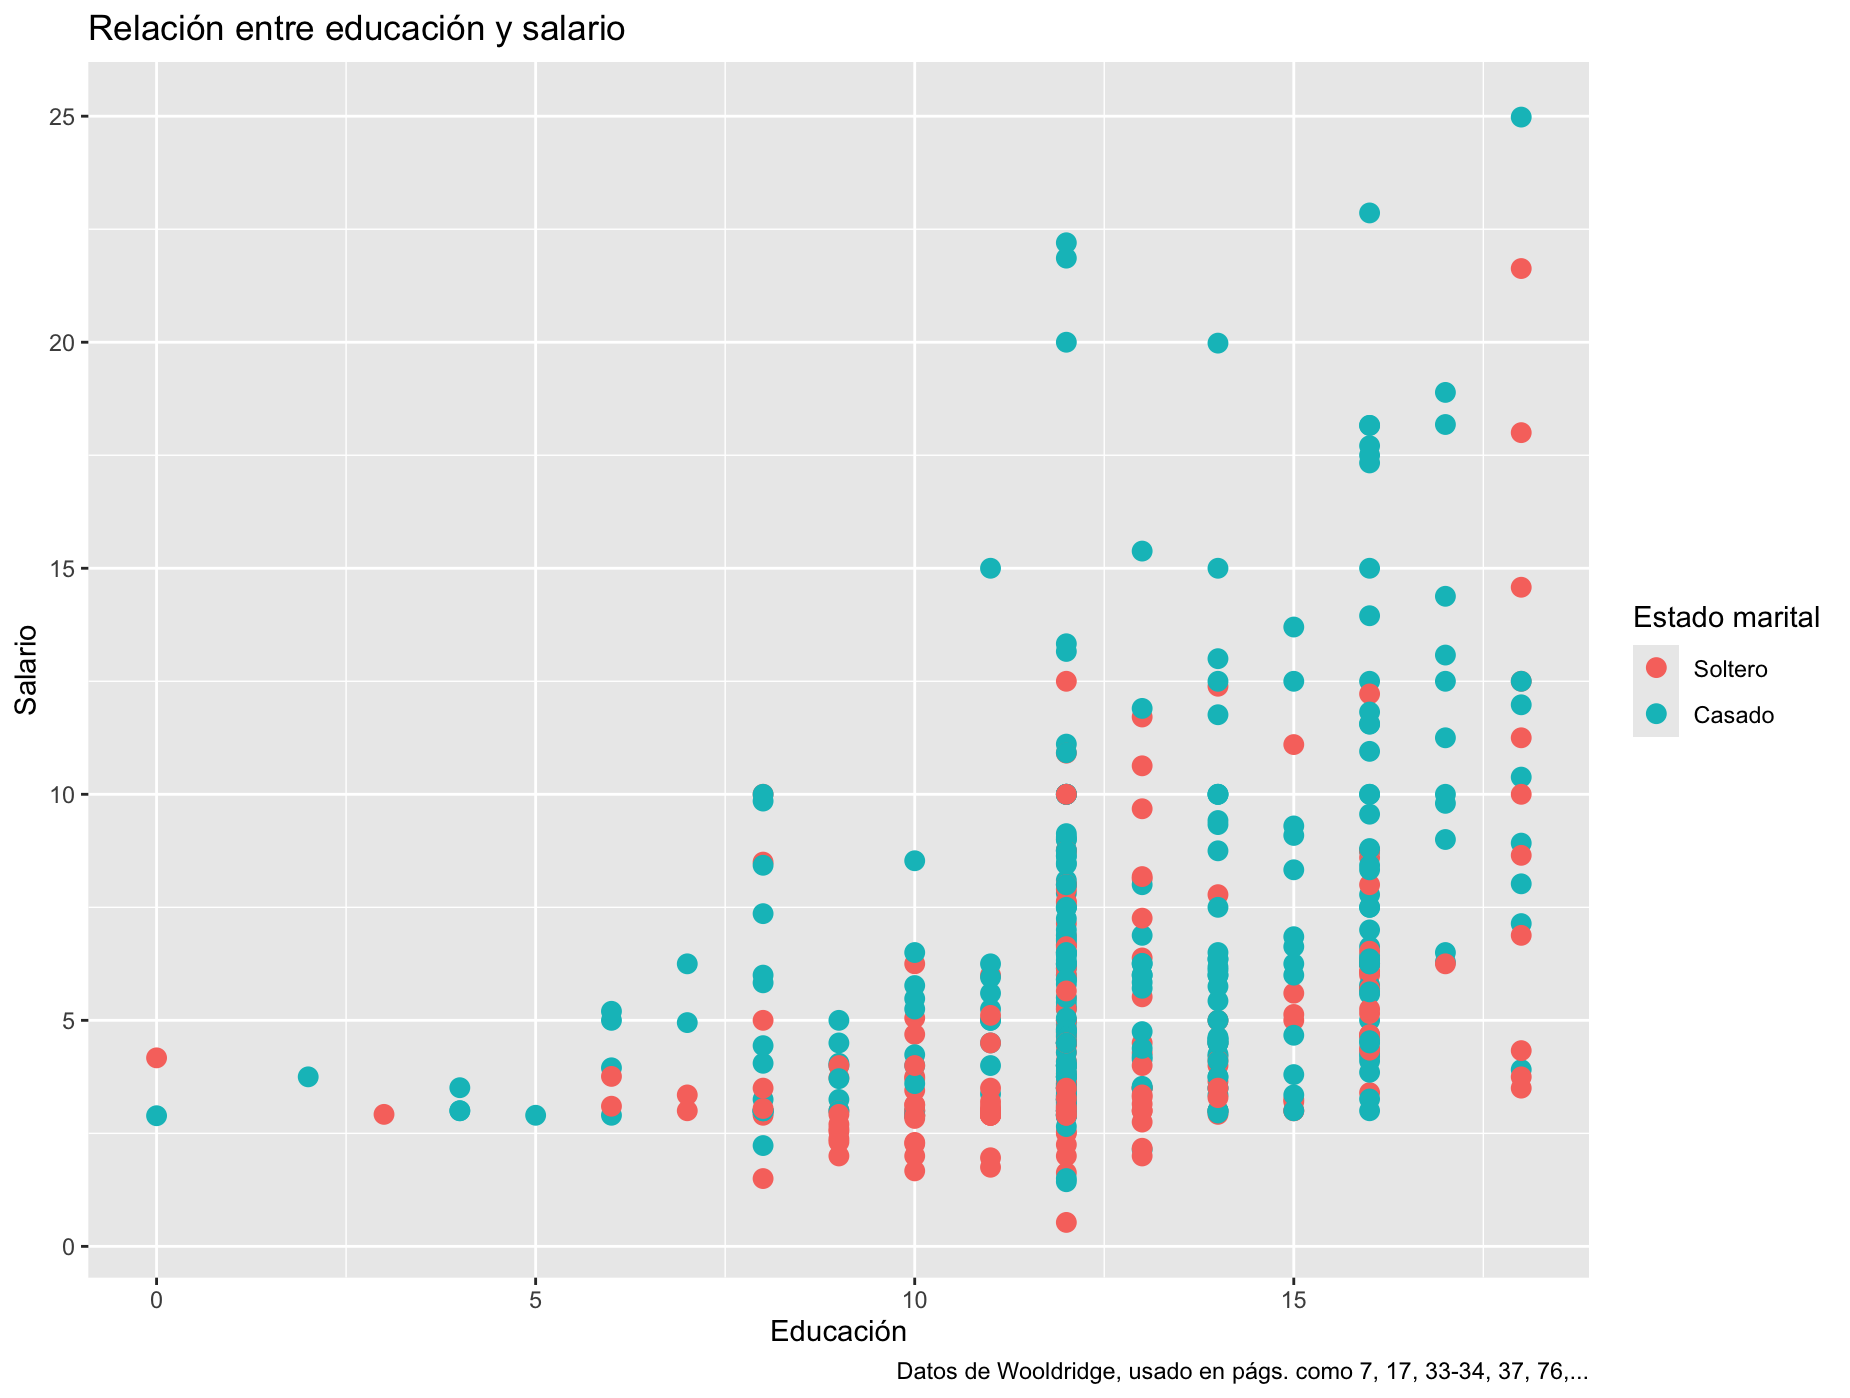
\includegraphics{Relación.png}
\caption{Meta 1: datos de ingreso, que continuaremos al abundar en
modelos inferenciales el sábado que viene.}
\end{figure}

Lo mismo podríamos hacer con los datos que trabajamos la semana pasada
de homicidios con armas de fuego en EEUU:

\begin{Shaded}
\begin{Highlighting}[]
\FunctionTok{library}\NormalTok{(dslabs)}
\FunctionTok{library}\NormalTok{(tidyverse)}
\end{Highlighting}
\end{Shaded}

\begin{verbatim}
## -- Attaching core tidyverse packages ------------------------ tidyverse 2.0.0 --
## v dplyr     1.1.4     v readr     2.1.5
## v forcats   1.0.0     v stringr   1.5.1
## v ggplot2   3.5.1     v tibble    3.2.1
## v lubridate 1.9.3     v tidyr     1.3.1
## v purrr     1.0.2     
## -- Conflicts ------------------------------------------ tidyverse_conflicts() --
## x dplyr::filter() masks stats::filter()
## x dplyr::lag()    masks stats::lag()
## i Use the conflicted package (<http://conflicted.r-lib.org/>) to force all conflicts to become errors
\end{verbatim}

\begin{Shaded}
\begin{Highlighting}[]
\FunctionTok{data}\NormalTok{(}\StringTok{"murders"}\NormalTok{)}
\FunctionTok{head}\NormalTok{(murders)}
\end{Highlighting}
\end{Shaded}

\begin{verbatim}
##        state abb region population total
## 1    Alabama  AL  South    4779736   135
## 2     Alaska  AK   West     710231    19
## 3    Arizona  AZ   West    6392017   232
## 4   Arkansas  AR  South    2915918    93
## 5 California  CA   West   37253956  1257
## 6   Colorado  CO   West    5029196    65
\end{verbatim}

No podemos determinar con facilidad a qué estado le toca la población
más grande o pequeña, y si existe alguna relación entre el tamaño de
población y el total de asesinatos, o de cómo varían las tasas de
asesinatos por regiones de estados en la federación estadounidense. Sin
embargo, eso puede responderse sin muchas palabras con el próximo
gráfico.

\begin{figure}
\centering
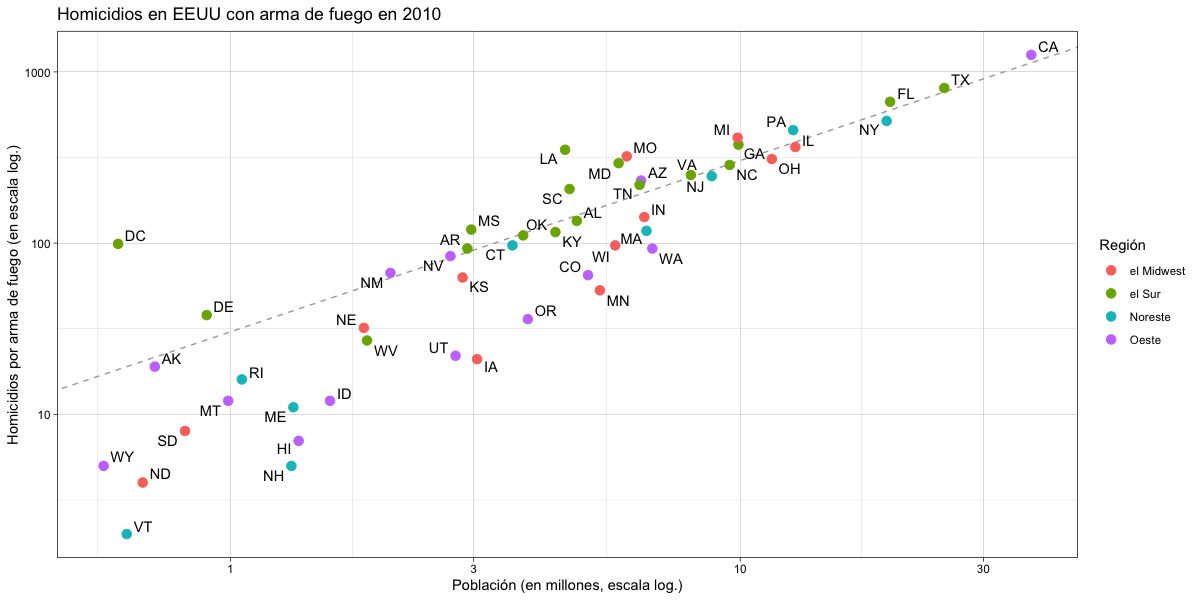
\includegraphics{Meta.png}
\caption{Gráfico de meta 2.}
\end{figure}

Una imagen vale más que mil palabras dice el dicho. Sin adentrarnos a la
inferencia estadística (que cubriremos en la tercera y última semana de
esta secuencia de talleres), hemos podido comunicar relaciones y
hallazgos en datos. A veces puede ser este ejercicio uno tan convincente
que no requiera análisis subsiguientes.

Vivimos en una era de creciente disponibilidad de conjuntos de datos
informativos y de herramientas de software, con lo cual el uso de
visualizaciones ha aumentado en diversos espacios: académicos,
gubernamentales, organizaciones sociales, prensa, e industrias varias.

En R, una de las principales maneras con la que trabajaremos estos
análisis visuales es de la mano de \texttt{ggplot2}, así como con otros
paquetes que ayudan a procesar esta información. Si bien existen otros
métodos de graficar en R y otros programas, la preferencia de este
taller es utilizar el sistema de procesamiento que ofrece
\texttt{tidyverse}, con \texttt{ggplot2} incluido.

Esta es una secuencia de tres semanas, y en esta lección continuamos con
lo aprendido la semana anterior, donde terminamos con visualizaciones
sencillas y con el uso de \texttt{tidyverse} para manejar datos. Tenemos
la meta hoy de que al culminar las segundas dos horas de esta secuencia
podamos:

\begin{enumerate}
\def\labelenumi{\arabic{enumi}.}
\item
  Entender cómo usar la gramática de gráficas
\item
  Entender cómo usar \texttt{ggplot2}, continuando con lo aprendido de
  \texttt{tidyverse} de la semana pasada.
\item
  Entender cómo utilizar en varias maneras \texttt{tidycensus} para
  generar mapas.
\end{enumerate}

La próxima sesión, del 18 de octubre, entraremos más en \emph{wrangling}
de datos, así como en la inferencia estadística, con introducciones en R
sobre modelos lineales, jerárquicos y longitudinales.

\section{ggplot2}\label{ggplot2}

R ofrece varias opciones para graficar, siendo útiles las capacidades
incluidas en su instalación básica. Además, existen paquetes como
\texttt{grid} y \texttt{lattice}. Sin embargo, en este taller (y en los
libros de referencia usados y descritos arriba) se ha optado por usar
\texttt{ggplot2}, ya que permite a los principiantes crear gráficos
complejos y estéticos mediante una sintaxis intuitiva y fácil de
recordar, dividiendo los gráficos en componentes básicos.

\texttt{ggplot2} destaca por su uso de una \emph{gramática de gráficos}
-- de donde vienen las primeras dos g -- que simplifica el proceso de
creación de gráficos. Al aprender unos pocos componentes esenciales de
esta gramática, los usuarios pueden generar una amplia variedad de
gráficos con facilidad. Además, su comportamiento por defecto está
diseñado para producir resultados agradables y funcionales con código
conciso y legible, lo que facilita su uso por principiantes. Como factor
limitante está el que está diseñado para trabajar con tablas de formato
\emph{tidy} (con filas con observaciones y columnas conteniendo
variables), pero un número sustancial de conjuntos de datos se trabajan
en ese formato, o pueden convertirse como tal.

\subsection{Componentes de un
gráfico}\label{componentes-de-un-gruxe1fico}

Hoy construiremos varios tipos de gráficos como los que vimos arriba,
así como mapas informativos. Antes que todo eso, vale señalar que los
gráficos se dividen en tres componentes principales. Usaré otro gráfico
que creara en 2020 durante la pandemia para ejemplificar estos
componentes.

\begin{figure}
\centering
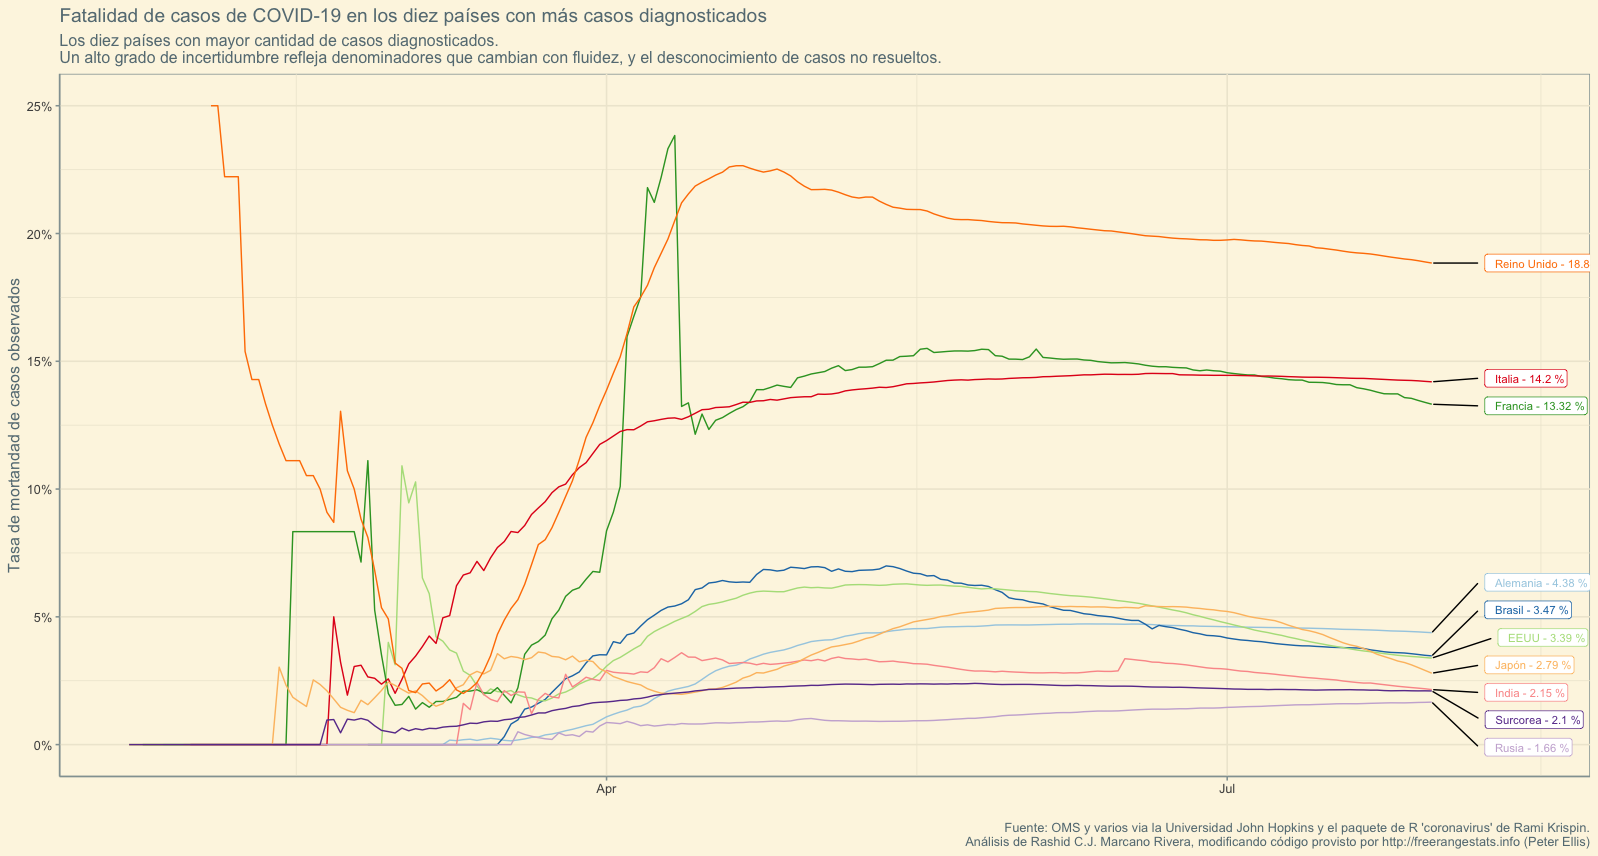
\includegraphics{Covid.png}
\caption{Datos para ejemplificar}
\end{figure}

\begin{itemize}
\tightlist
\item
  \textbf{Datos}:

  \begin{itemize}
  \tightlist
  \item
    Estoy pasando al gráfico un conjunto de datos que corté sobre
    fatalidad de casos de COVID-19 hasta el 31 de julio de 2020 (los
    datos continúan hasta 2023).\\
  \item
    Este es el componente de \emph{datos} del gráfico.
  \end{itemize}
\item
  \textbf{Geometrías}:

  \begin{itemize}
  \tightlist
  \item
    El gráfico es uno de líneas, útil para varias series de tiempo. Este
    componente es una geometría. Otras geometrías posibles son gráficos
    de dispersión, histogramas, diagramas de barras, densidades
    suavizadas, y diagrama de cajas, entre otros.\\
  \end{itemize}
\item
  \textbf{Mapeo estético}:

  \begin{itemize}
  \tightlist
  \item
    El gráfico usa señales visuales para representar en el lienzo vacío
    con capas distintos tipos de información provista en el conjunto de
    datos:

    \begin{itemize}
    \tightlist
    \item
      Posiciones en el eje de x (tiempo)\\
    \item
      Posiciones en el eje de y (tasas de mortandad observadas)\\
    \item
      Color (asignado por país)\\
    \end{itemize}
  \item
    Cada línea representa la información de un país para una serie de
    fechas. Estos se aclaran con una etiqueta para aclararnos esa
    relación de línea-color-país.\\
  \item
    El mapeo estético depende de la geometría utilizada.
  \end{itemize}
\item
  \textbf{Observaciones adicionales}:\\

  \begin{itemize}
  \tightlist
  \item
    Ejes x e y definidos por el rango de los datos y ambos en escalas
    logarítmicas.\\
  \item
    El gráfico incluye etiquetas, un título, etiquetas de variables,
    nota al calce, y el tema utilizado es uno solarizado que pareciera
    no muy distante al utilizado por el periódico ``Financial Times''.
  \end{itemize}
\item
  Volveremos luego a estos datos para construir esta imagen si nos da
  tiempo en el taller, y si no, tendrán disponible el cómo hacerlo para
  referencia.
\end{itemize}

\subsection{Lienzo vacío y capas}\label{lienzo-vacuxedo-y-capas}

Manteniéndonos cerca de los datos utilizados en la semana pasada,
construiremos por \textbf{\emph{capas}} la información que va en el
gráfico.

\begin{Shaded}
\begin{Highlighting}[]
\NormalTok{murders }\SpecialCharTok{|\textgreater{}} \FunctionTok{ggplot}\NormalTok{()}
\end{Highlighting}
\end{Shaded}

\includegraphics{Taller-2_files/figure-latex/Un lienzo en blanco-1.pdf}

El primer paso de crear un gráfico de ggplot es asignar los datos a un
lienzo vacío. Esto no significa poblar el lienzo con esos datos, sino
pasarle al programa la información inicial, como un pintor que
selecciona el tema que usará para la pintura que visualiza en su mente.
Esto lo hicimos al pasar el \emph{pipe}
(\texttt{\textbar{}\textgreater{}} o \texttt{\%\textgreater{}\%}) los
datos a ggplot, y lo que ocurrió fue que al no darle más información
(capas, como la pintura en un lienzo), nos quedó un recuadro gris
enmarcado por un borde blanco.

En ggplot, la información entonces se suministra al lienzo por capas, y
se le pueden añadir adicionales. Esto tomará la forma de código
siguiente:

DATOS \textbar\textgreater{} ggplot() + CAPA 1 + CAPA 2 + \ldots{} +
CAPA N

Usualmente, la primera capa que añadimos define la geometría. Si
queremos hacer un diagrama de dispersión, ¿qué geometría deberíamos
utilizar?

Si vemos la hoja de referencia (en la carpeta del taller 2, o accesible
en esta página:
\url{https://github.com/rstudio/cheatsheets/blob/main/data-visualization.pdf}),
vemos que la función utilizada para crear gráficos con esta geometría
puntillista es \texttt{geom\_point}.

\begin{Shaded}
\begin{Highlighting}[]
\NormalTok{murders }\SpecialCharTok{\%\textgreater{}\%}
  \FunctionTok{ggplot}\NormalTok{() }\SpecialCharTok{+}
  \FunctionTok{geom\_point}\NormalTok{(}\FunctionTok{aes}\NormalTok{(}\AttributeTok{x =}\NormalTok{ population}\SpecialCharTok{/}\DecValTok{10}\SpecialCharTok{\^{}}\DecValTok{6}\NormalTok{, }\AttributeTok{y =}\NormalTok{ total))}
\end{Highlighting}
\end{Shaded}

\includegraphics{Taller-2_files/figure-latex/Añadiendo una geometría-1.pdf}

En este caso ya hemos dado un paso adicional y añadido una primera capa
en esta obra: le indicamos que queremos una capa que tenga una geometría
de puntos, y un mapeo estético que toma las coordenadas en un plano
cartesiano donde el eje de equis queda definido como
\texttt{population/10\^{}6}, la población de los estados o Wáshington
D.C., en millones; el eje de ye queda definido entonces como el total de
asesinatos con armas de fuego. En el mapeo estético entonces los puntos
quedan asignados a esas coordenadas. De esta manera, las distancias
entre puntos, así como otras características que queramos añadir, quedan
expresadas. Esto se da a través de la función \texttt{aes}. Esta será de
las funciones que más usen al graficar.

Noten que hasta ahora hemos trabajado este lienzo sin guardarlo como
objeto. Si bien esto puede funcionar bien, es posible que queramos
guardar nuestro progreso y seguir añadiendo capas adicionales. En este
caso, al ejecutar el comando y guardarlo en objeto, el programa no nos
dará automáticamente una actualización del gráfico; tendremos que llamar
al objeto para que aparezca:

\begin{Shaded}
\begin{Highlighting}[]
\NormalTok{p}\OtherTok{\textless{}{-}}\NormalTok{murders }\SpecialCharTok{\%\textgreater{}\%}
  \FunctionTok{ggplot}\NormalTok{() }\SpecialCharTok{+}
  \FunctionTok{geom\_point}\NormalTok{(}\FunctionTok{aes}\NormalTok{(}\AttributeTok{x =}\NormalTok{ population}\SpecialCharTok{/}\DecValTok{10}\SpecialCharTok{\^{}}\DecValTok{6}\NormalTok{, }\AttributeTok{y =}\NormalTok{ total),}\AttributeTok{size=}\DecValTok{2}\NormalTok{)}

\NormalTok{p}
\end{Highlighting}
\end{Shaded}

\includegraphics{Taller-2_files/figure-latex/unnamed-chunk-2-1.pdf}

Tenemos entonces nuestro gráfico de dispersión inicial. Quizás no es tan
informativo pero vemos una serie de puntos con el mapeo estético
inicial. Noten que podríamos quitar la \texttt{x=} y la \texttt{y=} y no
pasaría nada, ya que en ausencia de esta especificación, el programa
entiende por defecto que lo primero que se le asigna es la información
del eje horizontal, y en segundo orden el vertical:

\begin{Shaded}
\begin{Highlighting}[]
\NormalTok{p}\SpecialCharTok{+}
  \FunctionTok{geom\_text}\NormalTok{(}\FunctionTok{aes}\NormalTok{(population}\SpecialCharTok{/}\DecValTok{10}\SpecialCharTok{\^{}}\DecValTok{6}\NormalTok{, total, }\AttributeTok{label =}\NormalTok{ abb))}
\end{Highlighting}
\end{Shaded}

\includegraphics{Taller-2_files/figure-latex/Añadiendo etiquetas-1.pdf}

Aquí he añadido una geometría nueva: texto. Hay dos geometrías para
esto, \texttt{geom\_label} y \texttt{geom\_text}, uno con el texto
enmarcado en un recuadro y el segundo sin ello. Ya que cada punto (cada
jurisdicción que es realmente parte de los Estados Unidos de América en
este caso) tiene una etiqueta, necesitamos un mapeo estético para hacer
la conexión entre los puntos y las etiquetas, así que se le asignó el
mismo tal que el texto cayera exactamente en la misma coordenada que el
punto. Pero esto se puede corregir:

\begin{Shaded}
\begin{Highlighting}[]
\NormalTok{p}\SpecialCharTok{+}
  \FunctionTok{geom\_text}\NormalTok{(}\FunctionTok{aes}\NormalTok{(population}\SpecialCharTok{/}\DecValTok{10}\SpecialCharTok{\^{}}\DecValTok{6}\NormalTok{, total, }\AttributeTok{label =}\NormalTok{ abb),}\AttributeTok{nudge\_x =} \FloatTok{1.5}\NormalTok{) }
\end{Highlighting}
\end{Shaded}

\includegraphics{Taller-2_files/figure-latex/Empujando etiquetas en el eje-1.pdf}

\begin{Shaded}
\begin{Highlighting}[]
\CommentTok{\#nudge\_y desplazaría el texto en el eje de y}
\end{Highlighting}
\end{Shaded}

En este caso hemos empujado a través del eje de equis la etiqueta de
texto con un valor numérico de 1.5. Valores mayores aumentarían la
distancia del texto y el punto, mientras que menores harían lo
contrario.

Ahora podremos seguir con una complicación en el mapeo estético:
queremos añadir una capa de color al lienzo que represente regiones de
estas jurisdicciones. Esto se hace al añadir la opción de
\texttt{colour} y dándole una variable, en este caso \texttt{region}.

\begin{Shaded}
\begin{Highlighting}[]
\CommentTok{\# Crear el gráfico base con puntos coloreados por región}
\NormalTok{p }\OtherTok{\textless{}{-}}\NormalTok{ murders }\SpecialCharTok{\%\textgreater{}\%}
  \FunctionTok{ggplot}\NormalTok{() }\SpecialCharTok{+}
  \FunctionTok{geom\_point}\NormalTok{(}\FunctionTok{aes}\NormalTok{(}\AttributeTok{x =}\NormalTok{ population}\SpecialCharTok{/}\DecValTok{10}\SpecialCharTok{\^{}}\DecValTok{6}\NormalTok{, }\AttributeTok{y =}\NormalTok{ total, }\AttributeTok{colour =}\NormalTok{ region), }\AttributeTok{size =} \DecValTok{2}\NormalTok{)}

\CommentTok{\# Mostrar el gráfico}
\NormalTok{p}
\end{Highlighting}
\end{Shaded}

\includegraphics{Taller-2_files/figure-latex/Añadiendo color-1.pdf}

Ahora paso nuevamente a añadir etiquetas abreviadas, con el color por
región.

\begin{Shaded}
\begin{Highlighting}[]
\CommentTok{\# Añadir etiquetas desplazadas en el eje x (con color por región)}
\NormalTok{p}\OtherTok{\textless{}{-}}\NormalTok{p }\SpecialCharTok{+} 
  \FunctionTok{geom\_text}\NormalTok{(}\FunctionTok{aes}\NormalTok{(}\AttributeTok{x =}\NormalTok{ population}\SpecialCharTok{/}\DecValTok{10}\SpecialCharTok{\^{}}\DecValTok{6}\NormalTok{, }\AttributeTok{y =}\NormalTok{ total, }\AttributeTok{label =}\NormalTok{ abb, }\AttributeTok{colour =}\NormalTok{ region), }\AttributeTok{nudge\_x =} \FloatTok{1.5}\NormalTok{)}
\NormalTok{p}
\end{Highlighting}
\end{Shaded}

\includegraphics{Taller-2_files/figure-latex/Añadiendo nuevamente etiquetas de abreviación jurisdiccional-1.pdf}

Y para darle más información al gráfico le añadimos etiquetas y títulos
que sean más informativas que los nombres de variables.

\begin{Shaded}
\begin{Highlighting}[]
\CommentTok{\#démosle más información a la gráfica de dispersión.}

\NormalTok{p}\SpecialCharTok{+}\FunctionTok{labs}\NormalTok{(}
  \AttributeTok{x =} \StringTok{"Población (en millones)"}\NormalTok{,   }\CommentTok{\# Cambia el nombre del eje x}
  \AttributeTok{y =} \StringTok{"Homicidios con arma de fuego"}\NormalTok{,            }\CommentTok{\# Cambia el nombre del eje y}
  \AttributeTok{colour =} \StringTok{"Región"}\NormalTok{,              }\CommentTok{\# Cambia el nombre de la leyenda de color}
  \AttributeTok{title =} \StringTok{"Homicidios con arma de fuego en EEUU, 2010"}  \CommentTok{\# Título del gráfico}
\NormalTok{)}
\end{Highlighting}
\end{Shaded}

\includegraphics{Taller-2_files/figure-latex/Añadiendo títulos-1.pdf}

Hasta ahora hemos ido añadiendo capas pero notamos que tenemos una gran
concentración de puntos en la parte inferior izquierda del lienzo: la
mayoría de las jurisdicciones tienen menos de 10 millones de habitantes
y menos de 400 homicidios. Esto hace leer e interpretar lo que sucede en
para estos casos difícil. Podríamos entonces representar el gráfico con
una transformación logarítmica al re-escalar con
\texttt{scale\_x\_continuous} y \texttt{scale\_y\_continuous}:

\begin{Shaded}
\begin{Highlighting}[]
\NormalTok{p2}\OtherTok{\textless{}{-}}\NormalTok{murders }\SpecialCharTok{\%\textgreater{}\%}
  \FunctionTok{ggplot}\NormalTok{() }\SpecialCharTok{+}
  \FunctionTok{geom\_point}\NormalTok{(}\FunctionTok{aes}\NormalTok{(}\AttributeTok{x =}\NormalTok{ population}\SpecialCharTok{/}\DecValTok{10}\SpecialCharTok{\^{}}\DecValTok{6}\NormalTok{, }\AttributeTok{y =}\NormalTok{ total, }\AttributeTok{colour =}\NormalTok{ region), }\AttributeTok{size =} \DecValTok{3}\NormalTok{)}
\NormalTok{p2}\OtherTok{\textless{}{-}}\NormalTok{ p2 }\SpecialCharTok{+} \FunctionTok{geom\_text}\NormalTok{(}\FunctionTok{aes}\NormalTok{(}\AttributeTok{x =}\NormalTok{ population}\SpecialCharTok{/}\DecValTok{10}\SpecialCharTok{\^{}}\DecValTok{6}\NormalTok{, }\AttributeTok{y =}\NormalTok{ total, }\AttributeTok{label =}\NormalTok{ abb),}\AttributeTok{nudge\_x =} \FloatTok{0.05}\NormalTok{)}
\NormalTok{p2}\OtherTok{\textless{}{-}}\NormalTok{p2}\SpecialCharTok{+}\FunctionTok{scale\_x\_continuous}\NormalTok{(}\AttributeTok{trans =} \StringTok{"log10"}\NormalTok{)}\SpecialCharTok{+}
  \FunctionTok{scale\_y\_continuous}\NormalTok{(}\AttributeTok{transform =} \StringTok{"log10"}\NormalTok{)}
\NormalTok{p2}\OtherTok{\textless{}{-}}\NormalTok{p2}\SpecialCharTok{+}
  \FunctionTok{labs}\NormalTok{(}
    \AttributeTok{x =} \StringTok{"Población (millones, escala log.)"}\NormalTok{,   }\CommentTok{\# Cambia el nombre del eje x}
    \AttributeTok{y =} \StringTok{"Homicidios por arma de fuego (escala log.)"}\NormalTok{,            }\CommentTok{\# Cambia el nombre del eje y}
    \AttributeTok{colour =} \StringTok{"Región"}\NormalTok{,              }\CommentTok{\# Cambia el nombre de la leyenda de color}
    \AttributeTok{title =} \StringTok{"Homicidios por arma de fuego vs población, por región"}  \CommentTok{\# Título del gráfico}
\NormalTok{  )}
\NormalTok{p2}
\end{Highlighting}
\end{Shaded}

\includegraphics{Taller-2_files/figure-latex/Haciendo una transformación de escala-1.pdf}

Podríamos añadir una capa temática, usando el paquete \texttt{ggthemes},
que tiene un catálogo estético variado, que recomiendo verifiquen a
través de
\url{https://yutannihilation.github.io/allYourFigureAreBelongToUs/ggthemes/}.
Esto es en adición a los que ya ofrece el paquete de \texttt{ggplot2}
\url{https://ggplot2.tidyverse.org/reference/ggtheme.html}.

En este caso le añadiré una visualización al estilo del semanario
británico \emph{The Economist.}

\begin{Shaded}
\begin{Highlighting}[]
\FunctionTok{library}\NormalTok{(ggthemes)}
\NormalTok{p2 }\SpecialCharTok{+} \FunctionTok{theme\_economist}\NormalTok{()}
\end{Highlighting}
\end{Shaded}

\includegraphics{Taller-2_files/figure-latex/Añadiendo temas-1.pdf}

\subsection{El gráfico que
buscábamos}\label{el-gruxe1fico-que-buscuxe1bamos}

Normalmente queremos añadir formas o anotaciones a las figuras que no se
derivan directamente del mapeo estético; algunos ejemplos incluyen
etiquetas, cuadros, áreas sombreadas y líneas. Si queremos añadir una
línea que represente la tasa promedio de asesinatos en todos los Estados
Unidos, tendremos que determinarlo aparte con la ayuda de \texttt{dplyr}
(parte de \texttt{tidyverse}), y tendremos que hacer la transformación
adecuada también (logarítmica):

\begin{Shaded}
\begin{Highlighting}[]
\FunctionTok{library}\NormalTok{(ggthemes)}
\FunctionTok{library}\NormalTok{(ggrepel)}
\end{Highlighting}
\end{Shaded}

\begin{verbatim}
## Warning: package 'ggrepel' was built under R version 4.3.3
\end{verbatim}

\begin{Shaded}
\begin{Highlighting}[]
\FunctionTok{library}\NormalTok{(dslabs)}
\NormalTok{t }\OtherTok{\textless{}{-}}\NormalTok{ murders }\SpecialCharTok{|\textgreater{}} 
  \FunctionTok{summarise}\NormalTok{(}\AttributeTok{tasa =} \FunctionTok{sum}\NormalTok{(total) }\SpecialCharTok{/}  \FunctionTok{sum}\NormalTok{(population) }\SpecialCharTok{*} \DecValTok{10}\SpecialCharTok{\^{}}\DecValTok{6}\NormalTok{) }\SpecialCharTok{|\textgreater{}}
  \FunctionTok{pull}\NormalTok{(tasa)}

\NormalTok{murders }\SpecialCharTok{|\textgreater{}} 
  \FunctionTok{mutate}\NormalTok{(región}\OtherTok{=}\FunctionTok{case\_when}\NormalTok{(}
\NormalTok{    region }\SpecialCharTok{==} \StringTok{"Northeast"} \SpecialCharTok{\textasciitilde{}} \StringTok{"Noreste"}\NormalTok{,}
\NormalTok{    region }\SpecialCharTok{==} \StringTok{"North Central"} \SpecialCharTok{\textasciitilde{}} \StringTok{"el Midwest"}\NormalTok{,}
\NormalTok{    region }\SpecialCharTok{==} \StringTok{"West"} \SpecialCharTok{\textasciitilde{}} \StringTok{"Oeste"}\NormalTok{,}
\NormalTok{    region }\SpecialCharTok{==} \StringTok{"South"} \SpecialCharTok{\textasciitilde{}} \StringTok{"el Sur"}\NormalTok{))}\SpecialCharTok{\%\textgreater{}\%}
  \FunctionTok{ggplot}\NormalTok{(}\FunctionTok{aes}\NormalTok{(population}\SpecialCharTok{/}\DecValTok{10}\SpecialCharTok{\^{}}\DecValTok{6}\NormalTok{, total)) }\SpecialCharTok{+}   
  \FunctionTok{geom\_abline}\NormalTok{(}\AttributeTok{intercept =} \FunctionTok{log10}\NormalTok{(t), }\AttributeTok{lty =} \DecValTok{2}\NormalTok{, }\AttributeTok{color =} \StringTok{"darkgrey"}\NormalTok{) }\SpecialCharTok{+}
  \FunctionTok{geom\_point}\NormalTok{(}\FunctionTok{aes}\NormalTok{(}\AttributeTok{col =}\NormalTok{ región), }\AttributeTok{size =} \DecValTok{3}\NormalTok{) }\SpecialCharTok{+}
  \FunctionTok{geom\_text\_repel}\NormalTok{(}\FunctionTok{aes}\NormalTok{(}\AttributeTok{label =}\NormalTok{ abb)) }\SpecialCharTok{+} 
  \FunctionTok{scale\_x\_log10}\NormalTok{() }\SpecialCharTok{+}
  \FunctionTok{scale\_y\_log10}\NormalTok{() }\SpecialCharTok{+}
  \FunctionTok{labs}\NormalTok{(}\AttributeTok{title =} \StringTok{"Homicidios en EEUU con arma de fuego en 2010"}\NormalTok{,}
       \AttributeTok{x =} \StringTok{"Población (en millones, escala log.)"}\NormalTok{, }
       \AttributeTok{y =} \StringTok{"Homicidios por arma de fuego (en escala log.)"}\NormalTok{,}
       \AttributeTok{color =} \StringTok{"Región"}\NormalTok{) }\SpecialCharTok{+}
  \FunctionTok{theme\_linedraw}\NormalTok{()}
\end{Highlighting}
\end{Shaded}

\includegraphics{Taller-2_files/figure-latex/el gráfico que buscábamos (datos de asesinatos)-1.pdf}

He aquí los pasos entonces que necesitábamos para recrear la imagen
arriba.'

\subsection{\texorpdfstring{Gráficos rápidos:
\texttt{qplot()}}{Gráficos rápidos: qplot()}}\label{gruxe1ficos-ruxe1pidos-qplot}

Si bien esto ha sido útil y han podido ver cómo generar gráficas
complejas siguiendo la gramática de gráficos, es probable que en algún
momento quieran ver rápidamente unas relaciones visuales de manera
instantánea, con la intención luego de volver y darle mejor forma y
seguir las complicaciones de un gráfico de \texttt{ggplot2} con todas
sus capas. La opción que da \texttt{ggplot2} a esto es el uso de
\texttt{qplot()}.

Por ejemplo, aquí modifiqué los grupos de jurisdicciones de Estados
Unidos a unos grupos específicos, y creo un gráfico para ver densidades
con relleno (\texttt{fill=grupo}) y con líneas que también sirven para
demarcar estos grupos de manera distinta (e.g.~línea sólida, línea
entrecortada). Noten que ha corrido todo el gráfico de la última línea.

\begin{Shaded}
\begin{Highlighting}[]
\NormalTok{murdersg}\OtherTok{\textless{}{-}}\NormalTok{murders }\SpecialCharTok{\%\textgreater{}\%}
  \FunctionTok{mutate}\NormalTok{(}\AttributeTok{tasa=}\NormalTok{ total}\SpecialCharTok{/}\NormalTok{population }\SpecialCharTok{*}\DecValTok{10}\SpecialCharTok{\^{}}\DecValTok{5}\NormalTok{,}
\NormalTok{    ,}\AttributeTok{grupo =} \FunctionTok{case\_when}\NormalTok{(}
\NormalTok{    abb }\SpecialCharTok{\%in\%} \FunctionTok{c}\NormalTok{(}\StringTok{"ME"}\NormalTok{, }\StringTok{"NH"}\NormalTok{, }\StringTok{"VT"}\NormalTok{, }\StringTok{"MA"}\NormalTok{, }\StringTok{"RI"}\NormalTok{, }\StringTok{"CT"}\NormalTok{) }\SpecialCharTok{\textasciitilde{}} \StringTok{"Nueva Inglaterra"}\NormalTok{,}
\NormalTok{    abb }\SpecialCharTok{\%in\%} \FunctionTok{c}\NormalTok{(}\StringTok{"WA"}\NormalTok{, }\StringTok{"OR"}\NormalTok{, }\StringTok{"CA"}\NormalTok{) }\SpecialCharTok{\textasciitilde{}} \StringTok{"Costa del Pacífico"}\NormalTok{,}
\NormalTok{    region }\SpecialCharTok{==} \StringTok{"South"} \SpecialCharTok{\textasciitilde{}} \StringTok{"el Sur"}\NormalTok{,}
    \ConstantTok{TRUE} \SpecialCharTok{\textasciitilde{}} \StringTok{"Otras regiones"}\NormalTok{))}
\FunctionTok{qplot}\NormalTok{(tasa, }\AttributeTok{data =}\NormalTok{ murdersg, }\AttributeTok{geom=} \StringTok{"density"}\NormalTok{, }\AttributeTok{fill =}\NormalTok{ grupo, }\AttributeTok{linetype=}\NormalTok{grupo)}
\end{Highlighting}
\end{Shaded}

\begin{verbatim}
## Warning: `qplot()` was deprecated in ggplot2 3.4.0.
## This warning is displayed once every 8 hours.
## Call `lifecycle::last_lifecycle_warnings()` to see where this warning was
## generated.
\end{verbatim}

\includegraphics{Taller-2_files/figure-latex/Un qplot inicial-1.pdf}

En las siguientes líneas pido y ejecuto variaciones de gráficos con
qplot con los datos de altura del libro de Irizarry:

\begin{Shaded}
\begin{Highlighting}[]
\FunctionTok{data}\NormalTok{(heights)            }
\NormalTok{b}\OtherTok{\textless{}{-}}\NormalTok{heights}\SpecialCharTok{|\textgreater{}}\FunctionTok{ggplot}\NormalTok{()}
\FunctionTok{qplot}\NormalTok{(sex, height, }\AttributeTok{data =}\NormalTok{ heights, }\AttributeTok{geom=} \StringTok{"boxplot"}\NormalTok{, }\AttributeTok{fill =}\NormalTok{ sex)}
\end{Highlighting}
\end{Shaded}

\includegraphics{Taller-2_files/figure-latex/Varios qplots-1.pdf}

\begin{Shaded}
\begin{Highlighting}[]
\FunctionTok{qplot}\NormalTok{(sex, height, }\AttributeTok{data =}\NormalTok{ heights, }\AttributeTok{geom=} \StringTok{"violin"}\NormalTok{, }\AttributeTok{fill =}\NormalTok{ sex)}
\end{Highlighting}
\end{Shaded}

\includegraphics{Taller-2_files/figure-latex/Varios qplots-2.pdf}

\begin{Shaded}
\begin{Highlighting}[]
\FunctionTok{qplot}\NormalTok{(sex, height, }\AttributeTok{data =}\NormalTok{ heights, }\AttributeTok{geom =} \StringTok{"dotplot"}\NormalTok{,}
      \AttributeTok{stackdir =} \StringTok{"center"}\NormalTok{, }\AttributeTok{binaxis =} \StringTok{"y"}\NormalTok{, }\AttributeTok{dotsize =} \FloatTok{0.3}\NormalTok{)}
\end{Highlighting}
\end{Shaded}

\begin{verbatim}
## Bin width defaults to 1/30 of the range of the data. Pick better value with
## `binwidth`.
\end{verbatim}

\includegraphics{Taller-2_files/figure-latex/Varios qplots-3.pdf}

\begin{Shaded}
\begin{Highlighting}[]
\FunctionTok{qplot}\NormalTok{(height, }\AttributeTok{data =}\NormalTok{ heights, }\AttributeTok{geom =} \StringTok{"density"}\NormalTok{, }\AttributeTok{fill =}\NormalTok{ sex)}
\end{Highlighting}
\end{Shaded}

\includegraphics{Taller-2_files/figure-latex/Varios qplots-4.pdf}

\begin{Shaded}
\begin{Highlighting}[]
\FunctionTok{qplot}\NormalTok{(height, }\AttributeTok{data =}\NormalTok{ heights, }\AttributeTok{geom =} \StringTok{"density"}\NormalTok{, }\AttributeTok{color =}\NormalTok{ sex, }\AttributeTok{linetype =}\NormalTok{ sex)}
\end{Highlighting}
\end{Shaded}

\includegraphics{Taller-2_files/figure-latex/Varios qplots-5.pdf}

Nuevamente podríamos mostrar información adicional, como medias añadidas
fuera de las estéticas definidas dentro del mapeo:

\begin{Shaded}
\begin{Highlighting}[]
\NormalTok{mu\_alt}\OtherTok{\textless{}{-}}\NormalTok{heights }\SpecialCharTok{\%\textgreater{}\%}
  \FunctionTok{group\_by}\NormalTok{(sex) }\SpecialCharTok{\%\textgreater{}\%}
  \FunctionTok{summarise}\NormalTok{(}\AttributeTok{media=}\FunctionTok{mean}\NormalTok{(height))}

\NormalTok{c}\OtherTok{\textless{}{-}}\NormalTok{heights}\SpecialCharTok{|\textgreater{}}\FunctionTok{ggplot}\NormalTok{(}\FunctionTok{aes}\NormalTok{(}\AttributeTok{x =}\NormalTok{ height))}
\NormalTok{c}\SpecialCharTok{+}\FunctionTok{geom\_density}\NormalTok{(}\FunctionTok{aes}\NormalTok{(}\AttributeTok{fill =}\NormalTok{ sex), }\AttributeTok{alpha=}\FloatTok{0.4}\NormalTok{) }\CommentTok{\#el alpha le da un nivel de transparencia }
\end{Highlighting}
\end{Shaded}

\includegraphics{Taller-2_files/figure-latex/Dando a densidades transparencias-1.pdf}

\begin{Shaded}
\begin{Highlighting}[]
\CommentTok{\#¿qué creen que pase si suben el valor a 0.9 o lo reducen a 0.1?}
\end{Highlighting}
\end{Shaded}

Noten que si tenemos dos categorías, al pedir color, tiende a establecer
a uno con un rojo magenta y al segundo con un azul cian (aciano o
ciano), en este caso suavizado y transparentado para poder ver las
distribuciones. Sin embargo, podemos editar el color manualmente, a la
vez que añadimos complicaciones como una media de alturas por grupo.

\begin{Shaded}
\begin{Highlighting}[]
\NormalTok{c}\SpecialCharTok{+} \FunctionTok{geom\_density}\NormalTok{(}\FunctionTok{aes}\NormalTok{(}\AttributeTok{color =}\NormalTok{ sex)) }\SpecialCharTok{+}
  \FunctionTok{geom\_vline}\NormalTok{(}\AttributeTok{data=}\NormalTok{mu\_alt, }\FunctionTok{aes}\NormalTok{(}\AttributeTok{xintercept=}\NormalTok{media, }\AttributeTok{color=}\NormalTok{sex),}
             \AttributeTok{linetype=}\StringTok{"dashed"}\NormalTok{) }\SpecialCharTok{+}
  \FunctionTok{scale\_color\_manual}\NormalTok{(}\AttributeTok{values=}\FunctionTok{c}\NormalTok{(}\StringTok{"\#999999"}\NormalTok{, }\StringTok{"\#E69F00"}\NormalTok{)) }\CommentTok{\#noten que aquí le di los colores con código alfanumérico, un gris plateado y un dorado.}
\end{Highlighting}
\end{Shaded}

\includegraphics{Taller-2_files/figure-latex/Añadiendo color manualmente-1.pdf}

Hay varios métodos para asignar colores al nombrarlos en R. Se puede
hacer por nombre (en inglés), con códigos alfanúmericos, y se puede
también importar paletas de colores con paquetes específicos. Considero
útil revisar las opciones en este enlace:
\url{https://r-graph-gallery.com/ggplot2-color.html}

\subsection{Alcanzando visualización de densidades y sus cambios a
través del
tiempo}\label{alcanzando-visualizaciuxf3n-de-densidades-y-sus-cambios-a-travuxe9s-del-tiempo}

\begin{Shaded}
\begin{Highlighting}[]
\FunctionTok{library}\NormalTok{(dslabs)}
\FunctionTok{data}\NormalTok{(gapminder)}
\NormalTok{gapminder }\SpecialCharTok{|\textgreater{}} \FunctionTok{as\_tibble}\NormalTok{()}
\end{Highlighting}
\end{Shaded}

\begin{verbatim}
## # A tibble: 10,545 x 9
##    country   year infant_mortality life_expectancy fertility population      gdp
##    <fct>    <int>            <dbl>           <dbl>     <dbl>      <dbl>    <dbl>
##  1 Albania   1960            115.             62.9      6.19    1636054 NA      
##  2 Algeria   1960            148.             47.5      7.65   11124892  1.38e10
##  3 Angola    1960            208              36.0      7.32    5270844 NA      
##  4 Antigua~  1960             NA              63.0      4.43      54681 NA      
##  5 Argenti~  1960             59.9            65.4      3.11   20619075  1.08e11
##  6 Armenia   1960             NA              66.9      4.55    1867396 NA      
##  7 Aruba     1960             NA              65.7      4.82      54208 NA      
##  8 Austral~  1960             20.3            70.9      3.45   10292328  9.67e10
##  9 Austria   1960             37.3            68.8      2.7     7065525  5.24e10
## 10 Azerbai~  1960             NA              61.3      5.57    3897889 NA      
## # i 10,535 more rows
## # i 2 more variables: continent <fct>, region <fct>
\end{verbatim}

Vemos que estos datos incluyen una variedad de información a nivel de
país, que incluye un número de años para ellos.

Podemos ver los grupos de países por continentes usando una matriz de
gráficos, con cuadrículas paradas y acostadas:

\begin{Shaded}
\begin{Highlighting}[]
\FunctionTok{filter}\NormalTok{(gapminder, year}\SpecialCharTok{\%in\%}\FunctionTok{c}\NormalTok{(}\DecValTok{1962}\NormalTok{, }\DecValTok{2012}\NormalTok{)) }\SpecialCharTok{|\textgreater{}}
  \FunctionTok{ggplot}\NormalTok{(}\FunctionTok{aes}\NormalTok{(fertility, life\_expectancy, }\AttributeTok{colour =}\NormalTok{ continent)) }\SpecialCharTok{+}
  \FunctionTok{geom\_point}\NormalTok{() }\SpecialCharTok{+}
  \FunctionTok{facet\_grid}\NormalTok{(continent}\SpecialCharTok{\textasciitilde{}}\NormalTok{year)}
\end{Highlighting}
\end{Shaded}

\includegraphics{Taller-2_files/figure-latex/unnamed-chunk-4-1.pdf}

\begin{Shaded}
\begin{Highlighting}[]
\FunctionTok{filter}\NormalTok{(gapminder, year}\SpecialCharTok{\%in\%}\FunctionTok{c}\NormalTok{(}\DecValTok{1962}\NormalTok{, }\DecValTok{2012}\NormalTok{)) }\SpecialCharTok{|\textgreater{}}
  \FunctionTok{ggplot}\NormalTok{(}\FunctionTok{aes}\NormalTok{(fertility, life\_expectancy, }\AttributeTok{col =}\NormalTok{ continent)) }\SpecialCharTok{+}
  \FunctionTok{geom\_point}\NormalTok{() }\SpecialCharTok{+}
  \FunctionTok{facet\_grid}\NormalTok{(. }\SpecialCharTok{\textasciitilde{}}\NormalTok{ year)}
\end{Highlighting}
\end{Shaded}

\includegraphics{Taller-2_files/figure-latex/unnamed-chunk-4-2.pdf}

\begin{Shaded}
\begin{Highlighting}[]
\NormalTok{years }\OtherTok{\textless{}{-}} \FunctionTok{c}\NormalTok{(}\DecValTok{1962}\NormalTok{, }\DecValTok{1980}\NormalTok{, }\DecValTok{1990}\NormalTok{, }\DecValTok{2000}\NormalTok{, }\DecValTok{2012}\NormalTok{,}\DecValTok{2015}\NormalTok{)}
\NormalTok{continents }\OtherTok{\textless{}{-}} \FunctionTok{c}\NormalTok{(}\StringTok{"Europe"}\NormalTok{, }\StringTok{"Asia"}\NormalTok{)}
\NormalTok{gapminder }\SpecialCharTok{|\textgreater{}}
  \FunctionTok{filter}\NormalTok{(year }\SpecialCharTok{\%in\%}\NormalTok{ years }\SpecialCharTok{\&}\NormalTok{ continent }\SpecialCharTok{\%in\%}\NormalTok{ continents) }\SpecialCharTok{|\textgreater{}}
  \FunctionTok{ggplot}\NormalTok{( }\FunctionTok{aes}\NormalTok{(fertility, life\_expectancy, }\AttributeTok{colour =}\NormalTok{ continent)) }\SpecialCharTok{+}
  \FunctionTok{geom\_point}\NormalTok{() }\SpecialCharTok{+}
  \FunctionTok{facet\_wrap}\NormalTok{(}\SpecialCharTok{\textasciitilde{}}\NormalTok{year)}\SpecialCharTok{+}\FunctionTok{labs}\NormalTok{(}\AttributeTok{x=}\StringTok{"Fertilidad"}\NormalTok{, }\AttributeTok{y=}\StringTok{"Esperanza de vida"}\NormalTok{,}\AttributeTok{colour=}\StringTok{"Continente"}\NormalTok{)}
\end{Highlighting}
\end{Shaded}

\includegraphics{Taller-2_files/figure-latex/unnamed-chunk-4-3.pdf}

En este caso podemos apreciar mejor cómo la dispersión y distribución de
países entre los años 1960s y el presente reciente ha ido encaminado a
una convergencia en estándares de vida, dejando atrás los puntos donde
originaron estereotipos que aún persisten sobre cómo son las vidas y
experiencias de distintas regiones del planeta (sin desestimar
diferencias e inequidades presentes).

\begin{Shaded}
\begin{Highlighting}[]
\NormalTok{gapminder }\OtherTok{\textless{}{-}}\NormalTok{ gapminder }\SpecialCharTok{|\textgreater{}} \FunctionTok{mutate}\NormalTok{(dólares}\AttributeTok{\_diarios =}\NormalTok{ gdp}\SpecialCharTok{/}\NormalTok{population}\SpecialCharTok{/}\DecValTok{365}\NormalTok{)}

\NormalTok{antaño }\OtherTok{\textless{}{-}} \DecValTok{1970}

\NormalTok{gapminder }\SpecialCharTok{|\textgreater{}}
  \FunctionTok{filter}\NormalTok{(year }\SpecialCharTok{==}\NormalTok{ antaño }\SpecialCharTok{\&} \SpecialCharTok{!}\FunctionTok{is.na}\NormalTok{(gdp)) }\SpecialCharTok{|\textgreater{}}
  \FunctionTok{mutate}\NormalTok{(}\AttributeTok{region =} \FunctionTok{reorder}\NormalTok{(region, dólares\_diarios, }\AttributeTok{FUN =}\NormalTok{ median)) }\SpecialCharTok{|\textgreater{}}
  \FunctionTok{ggplot}\NormalTok{(}\FunctionTok{aes}\NormalTok{(dólares\_diarios, region)) }\SpecialCharTok{+}
  \FunctionTok{geom\_point}\NormalTok{() }\SpecialCharTok{+}
  \FunctionTok{scale\_x\_continuous}\NormalTok{(}\AttributeTok{trans =} \StringTok{"log2"}\NormalTok{)}
\end{Highlighting}
\end{Shaded}

\includegraphics{Taller-2_files/figure-latex/Creando visualización sobre ingresos diarios-1.pdf}

\begin{Shaded}
\begin{Highlighting}[]
\NormalTok{gapminder }\OtherTok{\textless{}{-}}\NormalTok{ gapminder }\SpecialCharTok{|\textgreater{}}
  \FunctionTok{mutate}\NormalTok{(}\AttributeTok{grupo =} \FunctionTok{case\_when}\NormalTok{(}
\NormalTok{    region }\SpecialCharTok{\%in\%} \FunctionTok{c}\NormalTok{(}\StringTok{"Western Europe"}\NormalTok{, }\StringTok{"Northern Europe"}\NormalTok{,}\StringTok{"Southern Europe"}\NormalTok{,}
                  \StringTok{"Northern America"}\NormalTok{,}
                  \StringTok{"Australia and New Zealand"}\NormalTok{) }\SpecialCharTok{\textasciitilde{}} \StringTok{"Occidente"}\NormalTok{,}
\NormalTok{    region }\SpecialCharTok{\%in\%} \FunctionTok{c}\NormalTok{(}\StringTok{"Eastern Asia"}\NormalTok{, }\StringTok{"South{-}Eastern Asia"}\NormalTok{) }\SpecialCharTok{\textasciitilde{}} \StringTok{"Asia oriental"}\NormalTok{,}
\NormalTok{    region }\SpecialCharTok{\%in\%} \FunctionTok{c}\NormalTok{(}\StringTok{"Caribbean"}\NormalTok{, }\StringTok{"Central America"}\NormalTok{,}
                  \StringTok{"South America"}\NormalTok{) }\SpecialCharTok{\textasciitilde{}} \StringTok{"Latinoamérica"}\NormalTok{,}
\NormalTok{    continent }\SpecialCharTok{==} \StringTok{"Africa"} \SpecialCharTok{\&}
\NormalTok{      region }\SpecialCharTok{!=} \StringTok{"Northern Africa"} \SpecialCharTok{\textasciitilde{}} \StringTok{"África subsahariana"}\NormalTok{,}
    \ConstantTok{TRUE} \SpecialCharTok{\textasciitilde{}} \StringTok{"Otros"}\NormalTok{))}
\CommentTok{\#le damos orden a los niveles}
\NormalTok{gapminder }\OtherTok{\textless{}{-}}\NormalTok{ gapminder }\SpecialCharTok{|\textgreater{}}
  \FunctionTok{mutate}\NormalTok{(}\AttributeTok{grupo =} \FunctionTok{factor}\NormalTok{(grupo, }\AttributeTok{levels =} \FunctionTok{c}\NormalTok{(}\StringTok{"Otros"}\NormalTok{, }\StringTok{"Latinoamérica"}\NormalTok{,}
                                          \StringTok{"Asia oriental"}\NormalTok{, }\StringTok{"África subsahariana"}\NormalTok{,}
                                          \StringTok{"Occidente"}\NormalTok{)))}

\NormalTok{p }\OtherTok{\textless{}{-}}\NormalTok{ gapminder }\SpecialCharTok{|\textgreater{}}
  \FunctionTok{filter}\NormalTok{(year }\SpecialCharTok{==}\NormalTok{ antaño }\SpecialCharTok{\&} \SpecialCharTok{!}\FunctionTok{is.na}\NormalTok{(gdp)) }\SpecialCharTok{|\textgreater{}}
  \FunctionTok{ggplot}\NormalTok{(}\FunctionTok{aes}\NormalTok{(grupo, dólares\_diarios)) }\SpecialCharTok{+}
  \FunctionTok{geom\_boxplot}\NormalTok{() }\SpecialCharTok{+}
  \FunctionTok{scale\_y\_continuous}\NormalTok{(}\AttributeTok{trans =} \StringTok{"log2"}\NormalTok{) }\SpecialCharTok{+}
  \FunctionTok{xlab}\NormalTok{(}\StringTok{""}\NormalTok{) }\SpecialCharTok{+}
  \FunctionTok{theme}\NormalTok{(}\AttributeTok{axis.text.x =} \FunctionTok{element\_text}\NormalTok{(}\AttributeTok{angle =} \DecValTok{90}\NormalTok{, }\AttributeTok{hjust =} \DecValTok{1}\NormalTok{))}
\NormalTok{p}
\end{Highlighting}
\end{Shaded}

\includegraphics{Taller-2_files/figure-latex/Creando categorías para ver mejor dinámicas-1.pdf}

\begin{Shaded}
\begin{Highlighting}[]
\NormalTok{p }\SpecialCharTok{+} \FunctionTok{geom\_point}\NormalTok{(}\AttributeTok{alpha =} \FloatTok{0.5}\NormalTok{) }\CommentTok{\#añadiendo puntos para ver mejor distribuciones y cantidad de casos}
\end{Highlighting}
\end{Shaded}

\includegraphics{Taller-2_files/figure-latex/Creando categorías para ver mejor dinámicas-2.pdf}

\begin{Shaded}
\begin{Highlighting}[]
\FunctionTok{library}\NormalTok{(ggridges)}
\NormalTok{p }\OtherTok{\textless{}{-}}\NormalTok{ gapminder }\SpecialCharTok{|\textgreater{}}
  \FunctionTok{filter}\NormalTok{(year }\SpecialCharTok{==}\NormalTok{ antaño }\SpecialCharTok{\&} \SpecialCharTok{!}\FunctionTok{is.na}\NormalTok{(dólares\_diarios)) }\SpecialCharTok{|\textgreater{}}
  \FunctionTok{ggplot}\NormalTok{(}\FunctionTok{aes}\NormalTok{(dólares\_diarios, grupo)) }\SpecialCharTok{+}
  \FunctionTok{scale\_x\_continuous}\NormalTok{(}\AttributeTok{trans =} \StringTok{"log2"}\NormalTok{)}
\NormalTok{p }\SpecialCharTok{+} \FunctionTok{geom\_density\_ridges}\NormalTok{()}
\end{Highlighting}
\end{Shaded}

\begin{verbatim}
## Picking joint bandwidth of 0.648
\end{verbatim}

\includegraphics{Taller-2_files/figure-latex/Densidades-1.pdf}

\begin{Shaded}
\begin{Highlighting}[]
\NormalTok{p }\SpecialCharTok{+} \FunctionTok{geom\_density\_ridges}\NormalTok{(}\AttributeTok{jittered\_points =} \ConstantTok{TRUE}\NormalTok{,}
                        \AttributeTok{position =} \FunctionTok{position\_points\_jitter}\NormalTok{(}\AttributeTok{height =} \DecValTok{0}\NormalTok{),}
                        \AttributeTok{point\_shape =} \StringTok{\textquotesingle{}|\textquotesingle{}}\NormalTok{, }\AttributeTok{point\_size =} \DecValTok{3}\NormalTok{,}
                        \AttributeTok{point\_alpha =} \DecValTok{1}\NormalTok{, }\AttributeTok{alpha =} \FloatTok{0.7}\NormalTok{) }
\end{Highlighting}
\end{Shaded}

\begin{verbatim}
## Picking joint bandwidth of 0.648
\end{verbatim}

\includegraphics{Taller-2_files/figure-latex/Densidades con información de observaciones-1.pdf}

\begin{Shaded}
\begin{Highlighting}[]
\NormalTok{antaño }\OtherTok{\textless{}{-}} \DecValTok{1970}
\NormalTok{año\_presente }\OtherTok{\textless{}{-}} \DecValTok{2010}

\NormalTok{years }\OtherTok{\textless{}{-}} \FunctionTok{c}\NormalTok{(antaño, año\_presente)}
\NormalTok{gapminder }\SpecialCharTok{|\textgreater{}}
  \FunctionTok{filter}\NormalTok{(year }\SpecialCharTok{\%in\%}\NormalTok{ years }\SpecialCharTok{\&} \SpecialCharTok{!}\FunctionTok{is.na}\NormalTok{(gdp)) }\SpecialCharTok{|\textgreater{}}
  \FunctionTok{mutate}\NormalTok{(}\AttributeTok{west =} \FunctionTok{ifelse}\NormalTok{(grupo }\SpecialCharTok{==} \StringTok{"Occidente"}\NormalTok{, }\StringTok{"Occidente"}\NormalTok{, }\StringTok{"El Resto"}\NormalTok{)) }\SpecialCharTok{|\textgreater{}}
  \FunctionTok{ggplot}\NormalTok{(}\FunctionTok{aes}\NormalTok{(dólares\_diarios)) }\SpecialCharTok{+}
  \FunctionTok{geom\_histogram}\NormalTok{(}\AttributeTok{binwidth =} \DecValTok{1}\NormalTok{, }\AttributeTok{color =} \StringTok{"black"}\NormalTok{) }\SpecialCharTok{+}
  \FunctionTok{scale\_x\_continuous}\NormalTok{(}\AttributeTok{trans =} \StringTok{"log2"}\NormalTok{) }\SpecialCharTok{+}
  \FunctionTok{facet\_grid}\NormalTok{(year }\SpecialCharTok{\textasciitilde{}}\NormalTok{ west)}
\end{Highlighting}
\end{Shaded}

\includegraphics{Taller-2_files/figure-latex/Histogramas comparativos en facetas-1.pdf}
Sabemos que muchos países surgieron después de 1970 (razón por la cual
el histograma se nutre para el grupo \textbf{El Resto}), así que para
comparar los países que tienen toda la información y han existido
consistentemente entre esos periodos y ver si hay cambios y de dónde
surgen en distribuciones podemos hacer lo siguiente:

\begin{Shaded}
\begin{Highlighting}[]
\NormalTok{country\_list\_1 }\OtherTok{\textless{}{-}}\NormalTok{ gapminder }\SpecialCharTok{|\textgreater{}}
  \FunctionTok{filter}\NormalTok{(year }\SpecialCharTok{==}\NormalTok{ antaño }\SpecialCharTok{\&} \SpecialCharTok{!}\FunctionTok{is.na}\NormalTok{(dólares\_diarios)) }\SpecialCharTok{|\textgreater{}}
  \FunctionTok{pull}\NormalTok{(country)}

\NormalTok{country\_list\_2 }\OtherTok{\textless{}{-}}\NormalTok{ gapminder }\SpecialCharTok{|\textgreater{}}
  \FunctionTok{filter}\NormalTok{(year }\SpecialCharTok{==}\NormalTok{ año\_presente }\SpecialCharTok{\&} \SpecialCharTok{!}\FunctionTok{is.na}\NormalTok{(dólares\_diarios)) }\SpecialCharTok{|\textgreater{}}
  \FunctionTok{pull}\NormalTok{(country)}

\NormalTok{country\_list }\OtherTok{\textless{}{-}} \FunctionTok{intersect}\NormalTok{(country\_list\_1, country\_list\_2)}

\NormalTok{gapminder }\SpecialCharTok{|\textgreater{}}
  \FunctionTok{filter}\NormalTok{(year }\SpecialCharTok{\%in\%}\NormalTok{ years }\SpecialCharTok{\&}\NormalTok{ country }\SpecialCharTok{\%in\%}\NormalTok{ country\_list) }\SpecialCharTok{|\textgreater{}}
  \FunctionTok{ggplot}\NormalTok{(}\FunctionTok{aes}\NormalTok{(grupo, dólares\_diarios)) }\SpecialCharTok{+}
  \FunctionTok{geom\_boxplot}\NormalTok{() }\SpecialCharTok{+}
  \FunctionTok{theme}\NormalTok{(}\AttributeTok{axis.text.x =} \FunctionTok{element\_text}\NormalTok{(}\AttributeTok{angle =} \DecValTok{90}\NormalTok{, }\AttributeTok{hjust =} \DecValTok{1}\NormalTok{)) }\SpecialCharTok{+}
  \FunctionTok{scale\_y\_continuous}\NormalTok{(}\AttributeTok{trans =} \StringTok{"log2"}\NormalTok{) }\SpecialCharTok{+}
  \FunctionTok{xlab}\NormalTok{(}\StringTok{""}\NormalTok{) }\SpecialCharTok{+}
  \FunctionTok{facet\_grid}\NormalTok{(. }\SpecialCharTok{\textasciitilde{}}\NormalTok{ year)}
\end{Highlighting}
\end{Shaded}

\includegraphics{Taller-2_files/figure-latex/Wrangling para comparar chinas con chinas-1.pdf}

\begin{Shaded}
\begin{Highlighting}[]
\NormalTok{gapminder }\SpecialCharTok{|\textgreater{}}
  \FunctionTok{filter}\NormalTok{(year }\SpecialCharTok{\%in\%}\NormalTok{ years }\SpecialCharTok{\&} \SpecialCharTok{!}\FunctionTok{is.na}\NormalTok{(dólares\_diarios)) }\SpecialCharTok{|\textgreater{}}
  \FunctionTok{ggplot}\NormalTok{(}\FunctionTok{aes}\NormalTok{(dólares\_diarios, grupo)) }\SpecialCharTok{+}
  \FunctionTok{scale\_x\_continuous}\NormalTok{(}\AttributeTok{trans =} \StringTok{"log2"}\NormalTok{) }\SpecialCharTok{+}
  \FunctionTok{geom\_density\_ridges}\NormalTok{(}\AttributeTok{adjust =} \FloatTok{1.5}\NormalTok{) }\SpecialCharTok{+}
  \FunctionTok{facet\_grid}\NormalTok{(. }\SpecialCharTok{\textasciitilde{}}\NormalTok{ year)}
\end{Highlighting}
\end{Shaded}

\begin{verbatim}
## Warning in geom_density_ridges(adjust = 1.5): Ignoring unknown parameters:
## `adjust`
\end{verbatim}

\begin{verbatim}
## Picking joint bandwidth of 0.648
\end{verbatim}

\begin{verbatim}
## Picking joint bandwidth of 0.726
\end{verbatim}

\includegraphics{Taller-2_files/figure-latex/Wrangling para comparar chinas con chinas-2.pdf}

\begin{Shaded}
\begin{Highlighting}[]
\NormalTok{gapminder }\SpecialCharTok{|\textgreater{}}
  \FunctionTok{filter}\NormalTok{(year }\SpecialCharTok{\%in\%}\NormalTok{ years }\SpecialCharTok{\&}\NormalTok{ country }\SpecialCharTok{\%in\%}\NormalTok{ country\_list) }\SpecialCharTok{|\textgreater{}}
  \FunctionTok{group\_by}\NormalTok{(year) }\SpecialCharTok{|\textgreater{}}
  \FunctionTok{mutate}\NormalTok{(}\AttributeTok{weight =}\NormalTok{ population}\SpecialCharTok{/}\FunctionTok{sum}\NormalTok{(population)}\SpecialCharTok{*}\DecValTok{2}\NormalTok{) }\SpecialCharTok{|\textgreater{}}
  \FunctionTok{ungroup}\NormalTok{() }\SpecialCharTok{|\textgreater{}}
  \FunctionTok{ggplot}\NormalTok{(}\FunctionTok{aes}\NormalTok{(dólares\_diarios, }\AttributeTok{fill =}\NormalTok{ grupo)) }\SpecialCharTok{+}
  \FunctionTok{scale\_x\_continuous}\NormalTok{(}\AttributeTok{trans =} \StringTok{"log2"}\NormalTok{, }\AttributeTok{limit =} \FunctionTok{c}\NormalTok{(}\FloatTok{0.125}\NormalTok{, }\DecValTok{300}\NormalTok{)) }\SpecialCharTok{+}
  \FunctionTok{geom\_density}\NormalTok{(}\AttributeTok{alpha =} \FloatTok{0.2}\NormalTok{, }\AttributeTok{bw =} \FloatTok{0.75}\NormalTok{, }\AttributeTok{position =} \StringTok{"stack"}\NormalTok{) }\SpecialCharTok{+}
  \FunctionTok{facet\_grid}\NormalTok{(year }\SpecialCharTok{\textasciitilde{}}\NormalTok{ .)}\SpecialCharTok{+}\FunctionTok{labs}\NormalTok{(}\AttributeTok{title =} \StringTok{"Densidades apiladas: ingreso en dólares por día per cápita entre 1970 y 2010"}\NormalTok{,}
         \AttributeTok{x =} \StringTok{"Dólares por día"}\NormalTok{, }
         \AttributeTok{y =} \StringTok{"Densidad"}\NormalTok{,}
         \AttributeTok{color =} \StringTok{"Regiones"}\NormalTok{)}
\end{Highlighting}
\end{Shaded}

\includegraphics{Taller-2_files/figure-latex/Wrangling para comparar chinas con chinas-3.pdf}

\subsection{Datos del Covid}\label{datos-del-covid}

Durante la pandemia del Coronavirus de 2019, todos pasamos por bastantes
cosas, entre ellas, tratar de entender el fenómeno inaudito en nuestras
vidas, que era una mortífera y peligrosa pandemia, de la cual
desconocíamos en general muchas características. Esto llevó a los
gobiernos del mundo a tomar distintos tipos de acciones y nos
informábamos con gráficas así como números y tablas del progreso de la
enfermedad y su avance a través de los países del planeta, así como la
variable tasa de mortalidad que la acompañaba. Varios científicos
lanzaron programas para recoger y expresar estos datos al público
general para mantenernos todos bien informados.

En mi caso tomé código y datos que se recogían a menudo y produje por
unos meses varios tipos de gráficos para representar el desarrollo de la
pandemia (y tratar de entender qué ocurría de una manera que yo pudiera
digerir e informar). Aquí doy una versión del código que utilicé para
estos fines (modificando las fechas ya que se siguió recopilando esa
información mucho después de cuando dejara de actualizar esos gráficos.

\begin{Shaded}
\begin{Highlighting}[]
\CommentTok{\#devtools::install\_github("RamiKrispin/coronavirus",force = TRUE)}
\FunctionTok{library}\NormalTok{(coronavirus)}
\FunctionTok{library}\NormalTok{(scales)}
\end{Highlighting}
\end{Shaded}

\begin{verbatim}
## 
## Attaching package: 'scales'
\end{verbatim}

\begin{verbatim}
## The following object is masked from 'package:purrr':
## 
##     discard
\end{verbatim}

\begin{verbatim}
## The following object is masked from 'package:readr':
## 
##     col_factor
\end{verbatim}

\begin{Shaded}
\begin{Highlighting}[]
\NormalTok{coronavirus}\OtherTok{\textless{}{-}}\NormalTok{coronavirus}
\NormalTok{the\_caption }\OtherTok{=} \StringTok{"Fuente: OMS y varios via la Universidad John Hopkins y el paquete de R \textquotesingle{}coronavirus\textquotesingle{} de Rami Krispin.}\SpecialCharTok{\textbackslash{}n}\StringTok{Análisis de Rashid C.J. Marcano Rivera, modificando código provisto por http://freerangestats.info (Peter Ellis)"}
\NormalTok{top\_countries }\OtherTok{\textless{}{-}}\NormalTok{ coronavirus }\SpecialCharTok{\%\textgreater{}\%}
  \FunctionTok{filter}\NormalTok{(date }\SpecialCharTok{\textless{}=} \FunctionTok{as.Date}\NormalTok{(}\StringTok{"2020{-}07{-}31"}\NormalTok{)) }\SpecialCharTok{\%\textgreater{}\%}
  \FunctionTok{filter}\NormalTok{(type }\SpecialCharTok{==} \StringTok{"confirmed"}\NormalTok{) }\SpecialCharTok{\%\textgreater{}\%}
  \FunctionTok{group\_by}\NormalTok{(country) }\SpecialCharTok{\%\textgreater{}\%}
  \FunctionTok{summarise}\NormalTok{(}\AttributeTok{cases =} \FunctionTok{sum}\NormalTok{(cases)) }\SpecialCharTok{\%\textgreater{}\%}
  \FunctionTok{top\_n}\NormalTok{(}\DecValTok{10}\NormalTok{, }\AttributeTok{wt =}\NormalTok{ cases)}

\NormalTok{d2 }\OtherTok{\textless{}{-}}\NormalTok{ coronavirus }\SpecialCharTok{\%\textgreater{}\%}
  \FunctionTok{filter}\NormalTok{(date }\SpecialCharTok{\textless{}=} \FunctionTok{as.Date}\NormalTok{(}\StringTok{"2020{-}07{-}31"}\NormalTok{)) }\SpecialCharTok{\%\textgreater{}\%}  \CommentTok{\# Filtro para datos dentro de 2020}
  \FunctionTok{group\_by}\NormalTok{(date, country, type) }\SpecialCharTok{\%\textgreater{}\%}
  \FunctionTok{summarise}\NormalTok{(}\AttributeTok{cases =} \FunctionTok{sum}\NormalTok{(cases)) }\SpecialCharTok{\%\textgreater{}\%}
  \FunctionTok{group\_by}\NormalTok{(date, country) }\SpecialCharTok{\%\textgreater{}\%}
  \FunctionTok{spread}\NormalTok{(type, cases) }\SpecialCharTok{\%\textgreater{}\%}
  \FunctionTok{arrange}\NormalTok{(date) }\SpecialCharTok{\%\textgreater{}\%}
  \FunctionTok{group\_by}\NormalTok{(country) }\SpecialCharTok{\%\textgreater{}\%}
  \FunctionTok{mutate}\NormalTok{(}\AttributeTok{cfr\_cumulative =} \FunctionTok{cumsum}\NormalTok{(death) }\SpecialCharTok{/} \FunctionTok{cumsum}\NormalTok{(confirmed)) }\SpecialCharTok{\%\textgreater{}\%}
  \FunctionTok{filter}\NormalTok{(}\SpecialCharTok{!}\FunctionTok{is.na}\NormalTok{(cfr\_cumulative)) }\SpecialCharTok{\%\textgreater{}\%}
  \FunctionTok{ungroup}\NormalTok{() }\SpecialCharTok{\%\textgreater{}\%}
  \FunctionTok{inner\_join}\NormalTok{(top\_countries, }\AttributeTok{by =} \StringTok{"country"}\NormalTok{) }
\end{Highlighting}
\end{Shaded}

\begin{verbatim}
## `summarise()` has grouped output by 'date', 'country'. You can override using
## the `.groups` argument.
\end{verbatim}

\begin{Shaded}
\begin{Highlighting}[]
\FunctionTok{summary}\NormalTok{(}\FunctionTok{as.factor}\NormalTok{(d2}\SpecialCharTok{$}\NormalTok{country))}
\end{Highlighting}
\end{Shaded}

\begin{verbatim}
##         Brazil          Chile          India           Iran         Mexico 
##            157            160            184            164            155 
##           Peru         Russia   South Africa United Kingdom             US 
##            148            183            149            184            192
\end{verbatim}

\begin{Shaded}
\begin{Highlighting}[]
\NormalTok{today}\OtherTok{\textless{}{-}}\FunctionTok{as.Date}\NormalTok{(}\StringTok{"2020{-}08{-}06"}\NormalTok{)}
\NormalTok{x\_limits }\OtherTok{\textless{}{-}} \FunctionTok{c}\NormalTok{(today, }\ConstantTok{NA}\NormalTok{)}

\NormalTok{top\_countries}
\end{Highlighting}
\end{Shaded}

\begin{verbatim}
## # A tibble: 10 x 2
##    country          cases
##    <chr>            <dbl>
##  1 Brazil         2670451
##  2 Chile           355667
##  3 India          1695988
##  4 Iran            304204
##  5 Mexico          424637
##  6 Peru            407492
##  7 Russia          838461
##  8 South Africa    493183
##  9 US             4548497
## 10 United Kingdom  304789
\end{verbatim}

Vemos que los países están en inglés pero queremos que aparezcan en
nuestro gráfico en español (ya que interesa informar en mi caso a un
público hispanófono). Podemos modificar la información con los paquetes
de \texttt{tidyverse}:

\begin{Shaded}
\begin{Highlighting}[]
\NormalTok{d2}\OtherTok{\textless{}{-}}\NormalTok{ d2 }\SpecialCharTok{\%\textgreater{}\%}
  \FunctionTok{mutate}\NormalTok{(}\AttributeTok{country=}\FunctionTok{recode}\NormalTok{(country, }\AttributeTok{US =} \StringTok{"EEUU"}\NormalTok{, }\AttributeTok{Russia =}\StringTok{"Rusia"}\NormalTok{, }\AttributeTok{Mexico =} \StringTok{"México"}\NormalTok{, }\AttributeTok{Brazil =} \StringTok{"Brasil"}\NormalTok{, }
                        \StringTok{"United Kingdom"} \OtherTok{=} \StringTok{"Reino Unido"}\NormalTok{, }\AttributeTok{Japan=}\StringTok{"Japón"}\NormalTok{,}
                        \AttributeTok{Italy =} \StringTok{"Italia"}\NormalTok{, }\AttributeTok{Iran =} \StringTok{"Irán"}\NormalTok{, }\AttributeTok{Peru =} \StringTok{"Perú"}\NormalTok{,}
                        \StringTok{"South Africa"}\OtherTok{=} \StringTok{"Sudáfrica"}\NormalTok{))}
\NormalTok{d2}\OtherTok{\textless{}{-}}\NormalTok{ d2 }\SpecialCharTok{\%\textgreater{}\%}
  \FunctionTok{mutate}\NormalTok{(}\AttributeTok{cfr\_cumulativeperc=}\FunctionTok{round}\NormalTok{(cfr\_cumulative}\SpecialCharTok{*}\DecValTok{100}\NormalTok{,}\DecValTok{2}\NormalTok{))}
\end{Highlighting}
\end{Shaded}

Finalmente, expresamos el gráfico buscado. Paso los datos de mapeo
estético como opciones globales y le añado las capas: líneas para series
de tiempo, etiquetas automáticamente posicionadas (pero editadas para
especificar dónde las quiero y añadir información adicional),
transformaciones numéricas, información adicional de selección colores,
una extensión del marco para acomodar las etiquetas, así como los
títulos que deseara utilizar:

\begin{Shaded}
\begin{Highlighting}[]
\NormalTok{d2 }\SpecialCharTok{\%\textgreater{}\%}
  \FunctionTok{ggplot}\NormalTok{(}\FunctionTok{aes}\NormalTok{(}\AttributeTok{x =}\NormalTok{ date, }\AttributeTok{y =}\NormalTok{ cfr\_cumulative, }\AttributeTok{colour =}\NormalTok{ country)) }\SpecialCharTok{+}
  \FunctionTok{geom\_line}\NormalTok{() }\SpecialCharTok{+}
  \FunctionTok{geom\_label\_repel}\NormalTok{(}\AttributeTok{data =} \FunctionTok{filter}\NormalTok{(d2, date }\SpecialCharTok{==} \FunctionTok{max}\NormalTok{(date)), }\FunctionTok{aes}\NormalTok{(}\AttributeTok{label =} \FunctionTok{paste}\NormalTok{(}\StringTok{""}\NormalTok{,country,}\StringTok{"{-}"}\NormalTok{,cfr\_cumulativeperc,}\StringTok{"\%"}\NormalTok{)), }
                   \AttributeTok{hjust =} \DecValTok{1}\NormalTok{, }\AttributeTok{size =} \DecValTok{3}\NormalTok{, }\AttributeTok{xlim =}\NormalTok{ x\_limits, }\AttributeTok{segment.color=}\StringTok{"black"}\NormalTok{  ) }\SpecialCharTok{+}
  \FunctionTok{scale\_y\_continuous}\NormalTok{(}\AttributeTok{label =} \FunctionTok{percent\_format}\NormalTok{(}\AttributeTok{accuracy =} \DecValTok{1}\NormalTok{), }\AttributeTok{limits =} \FunctionTok{c}\NormalTok{(}\DecValTok{0}\NormalTok{, .}\DecValTok{25}\NormalTok{)) }\SpecialCharTok{+}
  \FunctionTok{scale\_colour\_brewer}\NormalTok{(}\AttributeTok{type =} \StringTok{\textquotesingle{}qual\textquotesingle{}}\NormalTok{, }\AttributeTok{palette =} \StringTok{\textquotesingle{}Paired\textquotesingle{}}\NormalTok{, }\AttributeTok{direction =} \DecValTok{1}\NormalTok{) }\SpecialCharTok{+}
  \FunctionTok{expand\_limits}\NormalTok{(}\AttributeTok{x =} \FunctionTok{max}\NormalTok{(d2}\SpecialCharTok{$}\NormalTok{date) }\SpecialCharTok{+} \DecValTok{13}\NormalTok{) }\SpecialCharTok{+}
  \FunctionTok{labs}\NormalTok{(}\AttributeTok{caption =}\NormalTok{ the\_caption,}
       \AttributeTok{x =} \StringTok{""}\NormalTok{,}
       \AttributeTok{y =} \StringTok{"Tasa de mortandad de casos observados"}\NormalTok{,}
       \AttributeTok{title =} \StringTok{"Fatalidad de casos de COVID{-}19 en los diez países con más casos diagnosticados"}\NormalTok{,}
       \AttributeTok{subtitle =} \StringTok{"Los diez países con mayor cantidad de casos diagnosticados. El caso de Irán ha sido truncado en sus primeras observaciones. }
\StringTok{Un alto grado de incertidumbre refleja denominadores que cambian con fluidez, y el desconocimiento de casos no resueltos."}\NormalTok{) }\SpecialCharTok{+}
  \FunctionTok{theme\_solarized}\NormalTok{()}\SpecialCharTok{+}  \FunctionTok{theme}\NormalTok{(}\AttributeTok{legend.position =} \StringTok{"none"}\NormalTok{)}
\end{Highlighting}
\end{Shaded}

\begin{verbatim}
## Warning: Removed 6 rows containing missing values or values outside the scale range
## (`geom_line()`).
\end{verbatim}

\includegraphics{Taller-2_files/figure-latex/Creando la visualización-1.pdf}

\section{Datos del censo}\label{datos-del-censo}

En este bloque introductorio, utilizamos los datos del Censo de Estados
Unidos para obtener variables demográficas y socioeconómicas de Puerto
Rico. Los datos del Censo nos permiten comprender mejor las
características de la población, como ingresos, educación, vivienda, y
más, a lo largo del tiempo. Para este ejercicio, hacemos uso de
\texttt{tidycensus}, una poderosa herramienta que facilita la descarga y
manipulación de los datos censales dentro del entorno de R.

El primer paso es cargar las bibliotecas necesarias, como
\texttt{tidyverse}, \texttt{tidycensus} y \texttt{sf}. La combinación de
estas bibliotecas nos permitirá no solo acceder a los datos, sino
también analizarlos y visualizarlos espacialmente en mapas. Es
importante también tener configurada una clave API de la Oficina del
Censo para poder acceder a los datos.

Luego, se configura el entorno con algunas opciones útiles:

\begin{itemize}
\item
  \texttt{scipen\ =\ 999}: Evita el uso de notación científica en los
  números, lo cual facilita la lectura de resultados.
\item
  \texttt{tigris\_class\ =\ "sf"}: Permite manejar las geometrías de
  manera eficiente mediante \texttt{sf}, una clase para manejar datos
  geoespaciales. A continuación, se usan las funciones de
  \texttt{tidycensus} para cargar variables específicas de diversos
  conjuntos de datos censales, como la Encuesta de la Comunidad
  Americana (ACS), la Encuesta de la Comunidad de Puerto Rico (PRCS, que
  se obtiene aquí vía la función de ACS) y los datos del Censo Decenal.
  Cada conjunto de datos proporciona información clave sobre diferentes
  periodos: anual, quinquenal y decenal. Finalmente, mostramos las
  variables disponibles que podemos utilizar para análisis posteriores.
\end{itemize}

\begin{Shaded}
\begin{Highlighting}[]
\FunctionTok{library}\NormalTok{(tidyverse)}
\FunctionTok{library}\NormalTok{(tidycensus)}
\end{Highlighting}
\end{Shaded}

\begin{verbatim}
## Warning: package 'tidycensus' was built under R version 4.3.3
\end{verbatim}

\begin{Shaded}
\begin{Highlighting}[]
\FunctionTok{library}\NormalTok{(sf)}
\end{Highlighting}
\end{Shaded}

\begin{verbatim}
## Warning: package 'sf' was built under R version 4.3.3
\end{verbatim}

\begin{verbatim}
## Linking to GEOS 3.11.0, GDAL 3.5.3, PROJ 9.1.0; sf_use_s2() is TRUE
\end{verbatim}

\begin{Shaded}
\begin{Highlighting}[]
\CommentTok{\#census\_api\_key(INSERTE SU LLAVE DEL CENSO AQUÍ)}
\FunctionTok{options}\NormalTok{(}\AttributeTok{scipen=}\DecValTok{999}\NormalTok{)}
\FunctionTok{options}\NormalTok{(}\AttributeTok{tigris\_class =} \StringTok{"sf"}\NormalTok{)}
\CommentTok{\#https://api.census.gov/data.html}
\NormalTok{census\_variables }\OtherTok{\textless{}{-}} \FunctionTok{load\_variables}\NormalTok{(}\AttributeTok{year =} \DecValTok{2020}\NormalTok{, }\AttributeTok{dataset =} \StringTok{"acs5"}\NormalTok{, }\AttributeTok{cache =} \ConstantTok{TRUE}\NormalTok{)}
\CommentTok{\#ensus\_variablessf1 \textless{}{-} load\_variables(year = 2020, dataset = "sf1", cache = TRUE)}
\CommentTok{\#census\_variablessf2 \textless{}{-} load\_variables(year = 2020, dataset = "sf2", cache = TRUE)}
\CommentTok{\#census\_variables4Redist \textless{}{-} load\_variables(year = 2020, dataset = "pl", cache = TRUE)}
\CommentTok{\#v00 \textless{}{-} load\_variables(2000, "sf3", cache = TRUE))}
\NormalTok{v18 }\OtherTok{\textless{}{-}} \FunctionTok{load\_variables}\NormalTok{(}\DecValTok{2018}\NormalTok{, }\StringTok{"acs5"}\NormalTok{, }\AttributeTok{cache =} \ConstantTok{TRUE}\NormalTok{)}
\NormalTok{v10 }\OtherTok{\textless{}{-}} \FunctionTok{load\_variables}\NormalTok{(}\DecValTok{2010}\NormalTok{, }\StringTok{"sf1"}\NormalTok{, }\AttributeTok{cache =} \ConstantTok{TRUE}\NormalTok{)}
\NormalTok{census\_variables}
\end{Highlighting}
\end{Shaded}

\begin{verbatim}
## # A tibble: 27,850 x 4
##    name        label                                    concept        geography
##    <chr>       <chr>                                    <chr>          <chr>    
##  1 B01001A_001 Estimate!!Total:                         SEX BY AGE (W~ tract    
##  2 B01001A_002 Estimate!!Total:!!Male:                  SEX BY AGE (W~ tract    
##  3 B01001A_003 Estimate!!Total:!!Male:!!Under 5 years   SEX BY AGE (W~ tract    
##  4 B01001A_004 Estimate!!Total:!!Male:!!5 to 9 years    SEX BY AGE (W~ tract    
##  5 B01001A_005 Estimate!!Total:!!Male:!!10 to 14 years  SEX BY AGE (W~ tract    
##  6 B01001A_006 Estimate!!Total:!!Male:!!15 to 17 years  SEX BY AGE (W~ tract    
##  7 B01001A_007 Estimate!!Total:!!Male:!!18 and 19 years SEX BY AGE (W~ tract    
##  8 B01001A_008 Estimate!!Total:!!Male:!!20 to 24 years  SEX BY AGE (W~ tract    
##  9 B01001A_009 Estimate!!Total:!!Male:!!25 to 29 years  SEX BY AGE (W~ tract    
## 10 B01001A_010 Estimate!!Total:!!Male:!!30 to 34 years  SEX BY AGE (W~ tract    
## # i 27,840 more rows
\end{verbatim}

\begin{Shaded}
\begin{Highlighting}[]
\NormalTok{v10}
\end{Highlighting}
\end{Shaded}

\begin{verbatim}
## # A tibble: 8,959 x 3
##    name    label                                concept         
##    <chr>   <chr>                                <chr>           
##  1 H001001 Total                                HOUSING UNITS   
##  2 H002001 Total                                URBAN AND RURAL 
##  3 H002002 Total!!Urban                         URBAN AND RURAL 
##  4 H002003 Total!!Urban!!Inside urbanized areas URBAN AND RURAL 
##  5 H002004 Total!!Urban!!Inside urban clusters  URBAN AND RURAL 
##  6 H002005 Total!!Rural                         URBAN AND RURAL 
##  7 H002006 Total!!Not defined for this file     URBAN AND RURAL 
##  8 H003001 Total                                OCCUPANCY STATUS
##  9 H003002 Total!!Occupied                      OCCUPANCY STATUS
## 10 H003003 Total!!Vacant                        OCCUPANCY STATUS
## # i 8,949 more rows
\end{verbatim}

\begin{Shaded}
\begin{Highlighting}[]
\NormalTok{v18}
\end{Highlighting}
\end{Shaded}

\begin{verbatim}
## # A tibble: 26,997 x 4
##    name        label                                  concept          geography
##    <chr>       <chr>                                  <chr>            <chr>    
##  1 B00001_001  Estimate!!Total                        UNWEIGHTED SAMP~ block gr~
##  2 B00002_001  Estimate!!Total                        UNWEIGHTED SAMP~ block gr~
##  3 B01001A_001 Estimate!!Total                        SEX BY AGE (WHI~ tract    
##  4 B01001A_002 Estimate!!Total!!Male                  SEX BY AGE (WHI~ tract    
##  5 B01001A_003 Estimate!!Total!!Male!!Under 5 years   SEX BY AGE (WHI~ tract    
##  6 B01001A_004 Estimate!!Total!!Male!!5 to 9 years    SEX BY AGE (WHI~ tract    
##  7 B01001A_005 Estimate!!Total!!Male!!10 to 14 years  SEX BY AGE (WHI~ tract    
##  8 B01001A_006 Estimate!!Total!!Male!!15 to 17 years  SEX BY AGE (WHI~ tract    
##  9 B01001A_007 Estimate!!Total!!Male!!18 and 19 years SEX BY AGE (WHI~ tract    
## 10 B01001A_008 Estimate!!Total!!Male!!20 to 24 years  SEX BY AGE (WHI~ tract    
## # i 26,987 more rows
\end{verbatim}

Podemos pasar por las variables en catálogo y seleccionar la que nos
llame más la atención. Recomiendo verifiquen las variables a través de
\texttt{View(variables)} ya que pueden usar una opción para filtrar e ir
buscando entre las miles de opciones que tienen para uso. En este caso,
quiero revisar para algún futuro trabajo de investigación datos sobre el
ingreso mediano de los distritos representativos de Puerto Rico para los
años 2018 y 2019 (que en el Censo aparecen como geografía tipo
\texttt{state\ legislative\ district\ (lower\ chamber)}). Usaré la
función \texttt{get\_acs}, podemos ver qué hace:

\begin{Shaded}
\begin{Highlighting}[]
\NormalTok{?get\_acs}
\FunctionTok{help}\NormalTok{(}\StringTok{"get\_acs"}\NormalTok{)}
\end{Highlighting}
\end{Shaded}

Para efectos estadísticos Puerto Rico entra como estado en estos datos.
Uso entonces la variable \texttt{B19013\_001} que da los ingresos
medianos por hogar.

\begin{Shaded}
\begin{Highlighting}[]
\NormalTok{prmedian\_2019 }\OtherTok{\textless{}{-}} \FunctionTok{get\_acs}\NormalTok{(}\AttributeTok{geography =} \StringTok{"state legislative district (lower chamber)"}\NormalTok{, }
              \AttributeTok{variables =} \FunctionTok{c}\NormalTok{(}\AttributeTok{medincome =} \StringTok{"B19013\_001"}\NormalTok{), }
              \AttributeTok{state =} \StringTok{"PR"}\NormalTok{, }
              \AttributeTok{year =} \DecValTok{2019}\NormalTok{)}
\end{Highlighting}
\end{Shaded}

\begin{verbatim}
## Getting data from the 2015-2019 5-year ACS
\end{verbatim}

\begin{Shaded}
\begin{Highlighting}[]
\NormalTok{prmedian\_2018 }\OtherTok{\textless{}{-}} \FunctionTok{get\_acs}\NormalTok{(}\AttributeTok{geography =} \StringTok{"state legislative district (lower chamber)"}\NormalTok{, }
                    \AttributeTok{variables =} \FunctionTok{c}\NormalTok{(}\AttributeTok{medincome =} \StringTok{"B19013\_001"}\NormalTok{), }
                    \AttributeTok{state =} \StringTok{"PR"}\NormalTok{, }
                    \AttributeTok{year =} \DecValTok{2018}\NormalTok{)}
\end{Highlighting}
\end{Shaded}

\begin{verbatim}
## Getting data from the 2014-2018 5-year ACS
\end{verbatim}

\begin{Shaded}
\begin{Highlighting}[]
\FunctionTok{head}\NormalTok{(prmedian\_2018)}
\end{Highlighting}
\end{Shaded}

\begin{verbatim}
## # A tibble: 6 x 5
##   GEOID NAME                                       variable  estimate   moe
##   <chr> <chr>                                      <chr>        <dbl> <dbl>
## 1 72001 State House District 1 (2018), Puerto Rico medincome    18336   955
## 2 72002 State House District 2 (2018), Puerto Rico medincome    18343   884
## 3 72003 State House District 3 (2018), Puerto Rico medincome    20315  1394
## 4 72004 State House District 4 (2018), Puerto Rico medincome    33471  1586
## 5 72005 State House District 5 (2018), Puerto Rico medincome    23274  1619
## 6 72006 State House District 6 (2018), Puerto Rico medincome    32921  1581
\end{verbatim}

\begin{Shaded}
\begin{Highlighting}[]
\NormalTok{pr\_median\_combined }\OtherTok{\textless{}{-}}\NormalTok{ prmedian\_2019 }\SpecialCharTok{\%\textgreater{}\%}
  \FunctionTok{mutate}\NormalTok{(}\AttributeTok{year =} \DecValTok{2019}\NormalTok{) }\SpecialCharTok{\%\textgreater{}\%}
  \FunctionTok{bind\_rows}\NormalTok{(}
\NormalTok{    prmedian\_2018 }\SpecialCharTok{\%\textgreater{}\%} \FunctionTok{mutate}\NormalTok{(}\AttributeTok{year =} \DecValTok{2018}\NormalTok{)}
\NormalTok{  )}
\FunctionTok{head}\NormalTok{(pr\_median\_combined)}
\end{Highlighting}
\end{Shaded}

\begin{verbatim}
## # A tibble: 6 x 6
##   GEOID NAME                                       variable estimate   moe  year
##   <chr> <chr>                                      <chr>       <dbl> <dbl> <dbl>
## 1 72001 State House District 1 (2018), Puerto Rico medinco~    18523  1142  2019
## 2 72002 State House District 2 (2018), Puerto Rico medinco~    19004   995  2019
## 3 72003 State House District 3 (2018), Puerto Rico medinco~    20655  1400  2019
## 4 72004 State House District 4 (2018), Puerto Rico medinco~    33678  1519  2019
## 5 72005 State House District 5 (2018), Puerto Rico medinco~    25912  1733  2019
## 6 72006 State House District 6 (2018), Puerto Rico medinco~    33977  1491  2019
\end{verbatim}

Habiendo obtenido las tablas, digamos que no quiero hacer sólo un
análisis numérico a ojo. El ojo y mente humana rara vez puede determinar
mucho al ver una colección grande de estos datos rápidamente.

Pero al visualizar, podemos mejorar algo la velocidad en lo que
entendemos algo más de lo que está ante nos.

\begin{Shaded}
\begin{Highlighting}[]
\NormalTok{pr\_median\_combined }\OtherTok{\textless{}{-}}\NormalTok{ pr\_median\_combined }\SpecialCharTok{\%\textgreater{}\%}
  \FunctionTok{filter}\NormalTok{(}\SpecialCharTok{!}\FunctionTok{is.na}\NormalTok{(estimate))  }\CommentTok{\# Filter out rows where the estimate is NA}

\NormalTok{pr\_median\_combined}\SpecialCharTok{|\textgreater{}}
  \FunctionTok{ggplot}\NormalTok{(}\FunctionTok{aes}\NormalTok{(}\AttributeTok{x =}\NormalTok{ NAME, }\AttributeTok{y =}\NormalTok{ estimate, }\AttributeTok{fill =} \FunctionTok{factor}\NormalTok{(year))) }\SpecialCharTok{+}
  \FunctionTok{geom\_bar}\NormalTok{(}\AttributeTok{stat =} \StringTok{"identity"}\NormalTok{, }\AttributeTok{position =} \FunctionTok{position\_dodge}\NormalTok{(), }\AttributeTok{color =} \StringTok{"black"}\NormalTok{) }\SpecialCharTok{+}
  \FunctionTok{geom\_errorbar}\NormalTok{(}\FunctionTok{aes}\NormalTok{(}\AttributeTok{ymin =}\NormalTok{ estimate }\SpecialCharTok{{-}}\NormalTok{ moe, }\AttributeTok{ymax =}\NormalTok{ estimate }\SpecialCharTok{+}\NormalTok{ moe), }
                \AttributeTok{position =} \FunctionTok{position\_dodge}\NormalTok{(}\FloatTok{0.9}\NormalTok{), }\AttributeTok{width =} \FloatTok{0.25}\NormalTok{) }\SpecialCharTok{+}
  \FunctionTok{scale\_y\_continuous}\NormalTok{(}\AttributeTok{labels =}\NormalTok{ scales}\SpecialCharTok{::}\FunctionTok{dollar\_format}\NormalTok{()) }\SpecialCharTok{+}
  \FunctionTok{labs}\NormalTok{(}
    \AttributeTok{title =} \StringTok{"Ingreso mediano por distrito legislativo en Puerto Rico (2018 vs 2019)"}\NormalTok{,}
    \AttributeTok{x =} \StringTok{"Distrito representativo"}\NormalTok{,}
    \AttributeTok{y =} \StringTok{"Ingreso mediano"}\NormalTok{,}
    \AttributeTok{fill =} \StringTok{"Año"}
\NormalTok{  ) }\SpecialCharTok{+}
  \FunctionTok{theme\_minimal}\NormalTok{() }\SpecialCharTok{+}
  \FunctionTok{theme}\NormalTok{(}
    \AttributeTok{axis.text.x =} \FunctionTok{element\_text}\NormalTok{(}\AttributeTok{angle =} \DecValTok{90}\NormalTok{, }\AttributeTok{vjust =} \FloatTok{0.5}\NormalTok{, }\AttributeTok{hjust =} \DecValTok{1}\NormalTok{)  }\CommentTok{\# Rotar nombres de distritos 90 grados para legibilidad}
\NormalTok{  )}
\end{Highlighting}
\end{Shaded}

\includegraphics{Taller-2_files/figure-latex/Ingresos por distrito, cambios en encuestas-1.pdf}

Noten que ordenó los distritos de una manera extraña: el 4 aparece antes
de 40 y todos del 5 al 9 se fueron como posteriores al 40. Voy a
corregir y renombrar los distritos:

\begin{Shaded}
\begin{Highlighting}[]
\NormalTok{pr\_median\_combined }\OtherTok{\textless{}{-}}\NormalTok{ pr\_median\_combined }\SpecialCharTok{\%\textgreater{}\%}
  \CommentTok{\# Extraer el número del distrito desde el nombre original y convertirlo en numérico}
  \FunctionTok{mutate}\NormalTok{(}\AttributeTok{district\_number =} \FunctionTok{as.numeric}\NormalTok{(}\FunctionTok{gsub}\NormalTok{(}\StringTok{".*District ([0{-}9]+).*"}\NormalTok{, }\StringTok{"}\SpecialCharTok{\textbackslash{}\textbackslash{}}\StringTok{1"}\NormalTok{, NAME))) }\SpecialCharTok{\%\textgreater{}\%}
  \CommentTok{\# Renombrar el campo NAME para que tenga el formato "Distrito 01" hasta "Distrito 40"}
  \FunctionTok{mutate}\NormalTok{(}\AttributeTok{NAME =} \FunctionTok{sprintf}\NormalTok{(}\StringTok{"Distrito \%02d"}\NormalTok{, district\_number)) }\SpecialCharTok{\%\textgreater{}\%}
  \CommentTok{\# Ordenar los datos según el número de distrito}
  \FunctionTok{arrange}\NormalTok{(district\_number)}

\CommentTok{\# Crear el gráfico nuevamente}
\NormalTok{pr\_median\_combined }\SpecialCharTok{|\textgreater{}}
  \FunctionTok{ggplot}\NormalTok{(}\FunctionTok{aes}\NormalTok{(}\AttributeTok{x =}\NormalTok{ NAME, }\AttributeTok{y =}\NormalTok{ estimate, }\AttributeTok{fill =} \FunctionTok{factor}\NormalTok{(year))) }\SpecialCharTok{+}
  \FunctionTok{geom\_bar}\NormalTok{(}\AttributeTok{stat =} \StringTok{"identity"}\NormalTok{, }\AttributeTok{position =} \FunctionTok{position\_dodge}\NormalTok{(), }\AttributeTok{color =} \StringTok{"black"}\NormalTok{) }\SpecialCharTok{+}
  \FunctionTok{geom\_errorbar}\NormalTok{(}\FunctionTok{aes}\NormalTok{(}\AttributeTok{ymin =}\NormalTok{ estimate }\SpecialCharTok{{-}}\NormalTok{ moe, }\AttributeTok{ymax =}\NormalTok{ estimate }\SpecialCharTok{+}\NormalTok{ moe), }
                \AttributeTok{position =} \FunctionTok{position\_dodge}\NormalTok{(}\FloatTok{0.9}\NormalTok{), }\AttributeTok{width =} \FloatTok{0.25}\NormalTok{) }\SpecialCharTok{+}
  \FunctionTok{scale\_y\_continuous}\NormalTok{(}\AttributeTok{labels =}\NormalTok{ scales}\SpecialCharTok{::}\FunctionTok{dollar\_format}\NormalTok{()) }\SpecialCharTok{+}
  \FunctionTok{labs}\NormalTok{(}
    \AttributeTok{title =} \StringTok{"Ingreso mediano por distrito representativo en Puerto Rico (2018 vs 2019)"}\NormalTok{,}
    \AttributeTok{x =} \StringTok{"Distrito representativo"}\NormalTok{,}
    \AttributeTok{y =} \StringTok{"Ingreso mediano"}\NormalTok{,}
    \AttributeTok{fill =} \StringTok{"Año"}
\NormalTok{  ) }\SpecialCharTok{+}
  \FunctionTok{theme\_minimal}\NormalTok{() }\SpecialCharTok{+}
  \FunctionTok{theme}\NormalTok{(}
    \AttributeTok{axis.text.x =} \FunctionTok{element\_text}\NormalTok{(}\AttributeTok{angle =} \DecValTok{90}\NormalTok{, }\AttributeTok{vjust =} \FloatTok{0.5}\NormalTok{, }\AttributeTok{hjust =} \DecValTok{1}\NormalTok{)  }\CommentTok{\# Rotar nombres de distritos 90 grados para legibilidad}
\NormalTok{  )}
\end{Highlighting}
\end{Shaded}

\includegraphics{Taller-2_files/figure-latex/Haciendo cambios a nombres de distritos-1.pdf}

Finalmente, usaremos esta información para generar un mapa geospacial
con ggplot. En este caso tomamos como parte de los pasos una
transformación de coordenadas para que el mapeo entienda dónde
posicionar las geometrías en el mapeo estético.

\begin{Shaded}
\begin{Highlighting}[]
\FunctionTok{library}\NormalTok{(tigris)}
\end{Highlighting}
\end{Shaded}

\begin{verbatim}
## To enable caching of data, set `options(tigris_use_cache = TRUE)`
## in your R script or .Rprofile.
\end{verbatim}

\begin{Shaded}
\begin{Highlighting}[]
\NormalTok{pr\_legislative\_districts }\OtherTok{\textless{}{-}} \FunctionTok{state\_legislative\_districts}\NormalTok{(}\AttributeTok{state =} \StringTok{"PR"}\NormalTok{, }\AttributeTok{house =} \StringTok{"lower"}\NormalTok{, }\AttributeTok{year =} \DecValTok{2018}\NormalTok{)}
\end{Highlighting}
\end{Shaded}

\begin{verbatim}
##   |                                                                              |                                                                      |   0%  |                                                                              |=                                                                     |   1%  |                                                                              |==                                                                    |   2%  |                                                                              |==                                                                    |   3%  |                                                                              |===                                                                   |   4%  |                                                                              |====                                                                  |   5%  |                                                                              |====                                                                  |   6%  |                                                                              |=====                                                                 |   7%  |                                                                              |======                                                                |   8%  |                                                                              |======                                                                |   9%  |                                                                              |=======                                                               |  10%  |                                                                              |========                                                              |  11%  |                                                                              |========                                                              |  12%  |                                                                              |=========                                                             |  13%  |                                                                              |==========                                                            |  14%  |                                                                              |==========                                                            |  15%  |                                                                              |===========                                                           |  16%  |                                                                              |============                                                          |  17%  |                                                                              |============                                                          |  18%  |                                                                              |=============                                                         |  19%  |                                                                              |==============                                                        |  19%  |                                                                              |==============                                                        |  20%  |                                                                              |===============                                                       |  21%  |                                                                              |===============                                                       |  22%  |                                                                              |================                                                      |  22%  |                                                                              |================                                                      |  23%  |                                                                              |=================                                                     |  24%  |                                                                              |==================                                                    |  25%  |                                                                              |==================                                                    |  26%  |                                                                              |===================                                                   |  27%  |                                                                              |====================                                                  |  28%  |                                                                              |====================                                                  |  29%  |                                                                              |=====================                                                 |  30%  |                                                                              |======================                                                |  31%  |                                                                              |======================                                                |  32%  |                                                                              |=======================                                               |  33%  |                                                                              |========================                                              |  34%  |                                                                              |========================                                              |  35%  |                                                                              |=========================                                             |  36%  |                                                                              |==========================                                            |  37%  |                                                                              |==========================                                            |  38%  |                                                                              |===========================                                           |  39%  |                                                                              |============================                                          |  39%  |                                                                              |============================                                          |  40%  |                                                                              |=============================                                         |  41%  |                                                                              |=============================                                         |  42%  |                                                                              |==============================                                        |  42%  |                                                                              |==============================                                        |  43%  |                                                                              |===============================                                       |  44%  |                                                                              |===============================                                       |  45%  |                                                                              |================================                                      |  45%  |                                                                              |================================                                      |  46%  |                                                                              |=================================                                     |  47%  |                                                                              |==================================                                    |  48%  |                                                                              |==================================                                    |  49%  |                                                                              |===================================                                   |  50%  |                                                                              |====================================                                  |  51%  |                                                                              |====================================                                  |  52%  |                                                                              |=====================================                                 |  53%  |                                                                              |======================================                                |  54%  |                                                                              |======================================                                |  55%  |                                                                              |=======================================                               |  56%  |                                                                              |========================================                              |  56%  |                                                                              |========================================                              |  57%  |                                                                              |=========================================                             |  58%  |                                                                              |=========================================                             |  59%  |                                                                              |==========================================                            |  59%  |                                                                              |==========================================                            |  60%  |                                                                              |===========================================                           |  61%  |                                                                              |===========================================                           |  62%  |                                                                              |============================================                          |  62%  |                                                                              |============================================                          |  63%  |                                                                              |=============================================                         |  64%  |                                                                              |=============================================                         |  65%  |                                                                              |==============================================                        |  65%  |                                                                              |==============================================                        |  66%  |                                                                              |===============================================                       |  67%  |                                                                              |===============================================                       |  68%  |                                                                              |================================================                      |  68%  |                                                                              |================================================                      |  69%  |                                                                              |=================================================                     |  70%  |                                                                              |=================================================                     |  71%  |                                                                              |==================================================                    |  71%  |                                                                              |==================================================                    |  72%  |                                                                              |===================================================                   |  73%  |                                                                              |===================================================                   |  74%  |                                                                              |====================================================                  |  74%  |                                                                              |=====================================================                 |  75%  |                                                                              |=====================================================                 |  76%  |                                                                              |======================================================                |  77%  |                                                                              |=======================================================               |  78%  |                                                                              |=======================================================               |  79%  |                                                                              |========================================================              |  80%  |                                                                              |=========================================================             |  81%  |                                                                              |=========================================================             |  82%  |                                                                              |==========================================================            |  83%  |                                                                              |===========================================================           |  84%  |                                                                              |===========================================================           |  85%  |                                                                              |============================================================          |  85%  |                                                                              |============================================================          |  86%  |                                                                              |=============================================================         |  87%  |                                                                              |=============================================================         |  88%  |                                                                              |==============================================================        |  88%  |                                                                              |==============================================================        |  89%  |                                                                              |===============================================================       |  90%  |                                                                              |===============================================================       |  91%  |                                                                              |================================================================      |  91%  |                                                                              |=================================================================     |  92%  |                                                                              |=================================================================     |  93%  |                                                                              |==================================================================    |  94%  |                                                                              |===================================================================   |  95%  |                                                                              |===================================================================   |  96%  |                                                                              |====================================================================  |  97%  |                                                                              |===================================================================== |  98%  |                                                                              |===================================================================== |  99%  |                                                                              |======================================================================| 100%
\end{verbatim}

\begin{Shaded}
\begin{Highlighting}[]
\NormalTok{pr\_legislative\_districts }\OtherTok{\textless{}{-}} \FunctionTok{st\_transform}\NormalTok{(pr\_legislative\_districts, }\AttributeTok{crs =} \StringTok{"EPSG:4326"}\NormalTok{)  }\CommentTok{\# ajustar proyección tal cual necesario}
\NormalTok{pr\_median\_2018\_geo }\OtherTok{\textless{}{-}}\NormalTok{ pr\_legislative\_districts }\SpecialCharTok{\%\textgreater{}\%}
  \FunctionTok{left\_join}\NormalTok{(prmedian\_2018, }\AttributeTok{by =} \FunctionTok{c}\NormalTok{(}\StringTok{"GEOID"} \OtherTok{=} \StringTok{"GEOID"}\NormalTok{))  }
\NormalTok{pr\_median\_2018\_geo}\SpecialCharTok{|\textgreater{}}
  \FunctionTok{ggplot}\NormalTok{() }\SpecialCharTok{+}
  \FunctionTok{geom\_sf}\NormalTok{(}\FunctionTok{aes}\NormalTok{(}\AttributeTok{fill =}\NormalTok{ estimate)) }\SpecialCharTok{+}
  \FunctionTok{scale\_fill\_viridis\_c}\NormalTok{(}\AttributeTok{option =} \StringTok{"plasma"}\NormalTok{, }\AttributeTok{name =} \StringTok{"Ingreso mediano"}\NormalTok{) }\SpecialCharTok{+}
  \FunctionTok{theme\_minimal}\NormalTok{() }\SpecialCharTok{+}
  \FunctionTok{labs}\NormalTok{(}
    \AttributeTok{title =} \StringTok{"Ingreso mediano por distrito representativo (2018)"}\NormalTok{,}
    \AttributeTok{fill =} \StringTok{"Ingreso mediano"}
\NormalTok{  )}
\end{Highlighting}
\end{Shaded}

\includegraphics{Taller-2_files/figure-latex/Ingreso mediano en mapa-1.pdf}

En este bloque próximo, utilizamos datos espaciales y demográficos para
mapear la población de Puerto Rico a nivel de tractos censales del censo
de 2020. Combinamos dos fuentes de información: una capa espacial con
los límites geográficos de los tractos (la forma de los polígonos en un
\emph{shapefile}:
\url{https://electionspuertorico.org/datos/2020/\#MAPA}) y los datos
poblacionales del Censo Decenal de 2020.

\begin{enumerate}
\def\labelenumi{\arabic{enumi}.}
\tightlist
\item
  El shapefile nos proporciona los límites de los tractos que
  necesitamos para asignar la información demográfica correctamente.
\end{enumerate}

\begin{itemize}
\item
  \textbf{\texttt{st\_read()}}: Carga el shapefile, aplicando la
  codificación~\texttt{latin1}~para asegurarnos de que los caracteres
  especiales (acentos, diéresis, eñes) en los nombres se lean
  correctamente.
\item
  \textbf{\texttt{st\_set\_crs()}~y~\texttt{st\_transform()}}: Aquí
  ajustamos el CRS (sistema de referencia de coordenadas) de la capa
  geográfica. Primero asignamos el CRS EPSG:4326 (coordenadas
  geográficas), y luego transformamos la capa a EPSG:3920 (un CRS
  proyectado que es común para Puerto Rico) para asegurar que todas las
  capas estén en el mismo sistema de referencia.
\end{itemize}

\begin{enumerate}
\def\labelenumi{\arabic{enumi}.}
\setcounter{enumi}{1}
\tightlist
\item
  \textbf{Datos de población}: Usamos~\texttt{tidycensus}~para obtener
  los datos de población de Puerto Rico a nivel de tractos censales del
  censo de 2020.

  \begin{itemize}
  \item
    \textbf{\texttt{get\_decennial()}}: Esta función descarga los datos
    de población (variable~\texttt{P1\_001N}, que representa el total de
    la población). La opción~\texttt{geometry\ =\ TRUE}~incluye la
    geometría de los tractos, lo cual nos permite hacer un análisis
    espacial directamente.
  \item
    \textbf{\texttt{st\_transform()}}: Aplicamos la misma transformación
    de CRS a los datos de población para que coincidan con la capa
    geográfica de los tractos.
  \end{itemize}
\item
  \textbf{Unión espacial}: Utilizamos~\texttt{st\_join()}~para combinar
  los datos espaciales y de población, uniendo la capa de tractos con
  los datos del censo según el campo~\texttt{GEOID}. Esto nos permite
  representar los datos poblacionales en el mapa.
\end{enumerate}

\begin{Shaded}
\begin{Highlighting}[]
\CommentTok{\# Este archivo lo descargué el 9 de agosto de 2022 desde https://electionspuertorico.org/datos/2020/PR2020TV.zip}
\NormalTok{folder}\OtherTok{\textless{}{-}}\StringTok{"\textasciitilde{}/Library/CloudStorage/OneDrive{-}IndianaUniversity/Elecciones/Rashid and Brevin/"}

\NormalTok{pr\_unidad\_shp\_filename }\OtherTok{\textless{}{-}} \FunctionTok{paste}\NormalTok{(folder, }\StringTok{"PR2020Shp/PR2020TV.shp"}\NormalTok{, }\AttributeTok{sep=} \StringTok{""}\NormalTok{)}
\NormalTok{pr\_unidades }\OtherTok{\textless{}{-}} \FunctionTok{st\_read}\NormalTok{(pr\_unidad\_shp\_filename, }\AttributeTok{options =} \StringTok{"ENCODING=latin1"}\NormalTok{)}
\end{Highlighting}
\end{Shaded}

\begin{verbatim}
## options:        ENCODING=latin1 
## Reading layer `PR2020TV' from data source 
##   `/Users/rashid/Library/CloudStorage/OneDrive-IndianaUniversity/Elecciones/Rashid and Brevin/PR2020Shp/PR2020TV.shp' 
##   using driver `ESRI Shapefile'
## Simple feature collection with 1365 features and 6 fields
## Geometry type: MULTIPOLYGON
## Dimension:     XY
## Bounding box:  xmin: -67.2713 ymin: 17.92684 xmax: -65.2442 ymax: 18.51609
## Geodetic CRS:  WGS 84
\end{verbatim}

\begin{Shaded}
\begin{Highlighting}[]
\FunctionTok{st\_set\_crs}\NormalTok{(pr\_unidades, }\StringTok{"EPSG:4326"}\NormalTok{)}
\end{Highlighting}
\end{Shaded}

\begin{verbatim}
## Simple feature collection with 1365 features and 6 fields
## Geometry type: MULTIPOLYGON
## Dimension:     XY
## Bounding box:  xmin: -67.2713 ymin: 17.92684 xmax: -65.2442 ymax: 18.51609
## Geodetic CRS:  WGS 84
## First 10 features:
##       Municipio Precinto Unidad Grupo DS DR                       geometry
## 1  Barranquitas       70      5     3  6 26 MULTIPOLYGON (((-66.30361 1...
## 2     Cabo Rojo       46      2     3  4 20 MULTIPOLYGON (((-67.14746 1...
## 3     Cabo Rojo       46      3     3  4 20 MULTIPOLYGON (((-67.16632 1...
## 4     Cabo Rojo       46      9     2  4 20 MULTIPOLYGON (((-67.1375 18...
## 5     Cabo Rojo       46      6     3  4 20 MULTIPOLYGON (((-67.16957 1...
## 6    San Germán       44      3     1  4 20 MULTIPOLYGON (((-67.08108 1...
## 7    San Germán       43      7     2  4 19 MULTIPOLYGON (((-67.02885 1...
## 8    San Germán       43      6     2  4 19 MULTIPOLYGON (((-67.04865 1...
## 9    San Germán       44      4     1  4 20 MULTIPOLYGON (((-67.06009 1...
## 10   San Germán       43      2     1  4 19 MULTIPOLYGON (((-67.08731 1...
\end{verbatim}

\begin{Shaded}
\begin{Highlighting}[]
\NormalTok{pr\_unidades }\OtherTok{\textless{}{-}}\NormalTok{ pr\_unidades }\SpecialCharTok{\%\textgreater{}\%} \FunctionTok{st\_transform}\NormalTok{(}\AttributeTok{crs =} \StringTok{"EPSG:3920"}\NormalTok{)}
\FunctionTok{plot}\NormalTok{(pr\_unidades)}
\end{Highlighting}
\end{Shaded}

\includegraphics{Taller-2_files/figure-latex/unnamed-chunk-6-1.pdf}

\begin{Shaded}
\begin{Highlighting}[]
\NormalTok{pr\_population }\OtherTok{\textless{}{-}} \FunctionTok{get\_decennial}\NormalTok{(}
  \AttributeTok{geography =} \StringTok{"tract"}\NormalTok{, }
  \AttributeTok{variables =} \StringTok{"P1\_001N"}\NormalTok{, }
  \AttributeTok{state =} \StringTok{"72"}\NormalTok{,   }\CommentTok{\# FIPS code for Puerto Rico}
  \AttributeTok{year =} \DecValTok{2020}\NormalTok{, }
  \AttributeTok{geometry =} \ConstantTok{TRUE}
\NormalTok{)}
\end{Highlighting}
\end{Shaded}

\begin{verbatim}
## Getting data from the 2020 decennial Census
\end{verbatim}

\begin{verbatim}
## Downloading feature geometry from the Census website.  To cache shapefiles for use in future sessions, set `options(tigris_use_cache = TRUE)`.
\end{verbatim}

\begin{verbatim}
## Using the PL 94-171 Redistricting Data Summary File
\end{verbatim}

\begin{verbatim}
##   |                                                                              |                                                                      |   0%  |                                                                              |==                                                                    |   3%  |                                                                              |====                                                                  |   5%  |                                                                              |======                                                                |   8%  |                                                                              |========                                                              |  11%  |                                                                              |==========                                                            |  14%  |                                                                              |===========                                                           |  16%  |                                                                              |=============                                                         |  19%  |                                                                              |===============                                                       |  22%  |                                                                              |=================                                                     |  25%  |                                                                              |===================                                                   |  27%  |                                                                              |=====================                                                 |  30%  |                                                                              |=======================                                               |  33%  |                                                                              |=========================                                             |  35%  |                                                                              |===========================                                           |  38%  |                                                                              |=============================                                         |  41%  |                                                                              |==============================                                        |  43%  |                                                                              |================================                                      |  46%  |                                                                              |==================================                                    |  48%  |                                                                              |====================================                                  |  51%  |                                                                              |======================================                                |  54%  |                                                                              |========================================                              |  57%  |                                                                              |==========================================                            |  59%  |                                                                              |===========================================                           |  62%  |                                                                              |=============================================                         |  65%  |                                                                              |===============================================                       |  68%  |                                                                              |=================================================                     |  70%  |                                                                              |===================================================                   |  73%  |                                                                              |=====================================================                 |  76%  |                                                                              |=======================================================               |  78%  |                                                                              |=========================================================             |  81%  |                                                                              |===========================================================           |  84%  |                                                                              |=============================================================         |  86%  |                                                                              |==============================================================        |  89%  |                                                                              |================================================================      |  92%  |                                                                              |==================================================================    |  95%  |                                                                              |====================================================================  |  97%  |                                                                              |======================================================================| 100%
\end{verbatim}

\begin{verbatim}
## Note: 2020 decennial Census data use differential privacy, a technique that
## introduces errors into data to preserve respondent confidentiality.
## i Small counts should be interpreted with caution.
## i See https://www.census.gov/library/fact-sheets/2021/protecting-the-confidentiality-of-the-2020-census-redistricting-data.html for additional guidance.
## This message is displayed once per session.
\end{verbatim}

\begin{Shaded}
\begin{Highlighting}[]
\NormalTok{pr\_population }\OtherTok{\textless{}{-}} \FunctionTok{st\_transform}\NormalTok{(pr\_population, }\AttributeTok{crs =} \StringTok{"EPSG:3920"}\NormalTok{)}
\NormalTok{pr\_unidades }\OtherTok{\textless{}{-}}\NormalTok{ pr\_unidades }\SpecialCharTok{\%\textgreater{}\%}
  \FunctionTok{st\_join}\NormalTok{(pr\_population, }\AttributeTok{by =} \FunctionTok{c}\NormalTok{(}\StringTok{"GEOID"} \OtherTok{=} \StringTok{"GEOID"}\NormalTok{))  }\CommentTok{\# Asumiendo que comparten GEOID en común}
\NormalTok{pr\_unidades}\SpecialCharTok{|\textgreater{}}\FunctionTok{ggplot}\NormalTok{() }\SpecialCharTok{+}
  \FunctionTok{geom\_sf}\NormalTok{(}\FunctionTok{aes}\NormalTok{(}\AttributeTok{fill =}\NormalTok{ value)) }\SpecialCharTok{+}  \CommentTok{\# \textasciigrave{}value\textasciigrave{} is the population count}
  \FunctionTok{scale\_fill\_viridis\_c}\NormalTok{(}\AttributeTok{option =} \StringTok{"plasma"}\NormalTok{, }\AttributeTok{name =} \StringTok{"Population"}\NormalTok{) }\SpecialCharTok{+}
  \FunctionTok{theme\_minimal}\NormalTok{() }\SpecialCharTok{+}
  \FunctionTok{labs}\NormalTok{(}\AttributeTok{title =} \StringTok{"Población de Puerto Rico por tracto censal (2020)"}\NormalTok{)}
\end{Highlighting}
\end{Shaded}

\includegraphics{Taller-2_files/figure-latex/Población-1.pdf}

\begin{Shaded}
\begin{Highlighting}[]
\NormalTok{pr\_unidades}
\end{Highlighting}
\end{Shaded}

\begin{verbatim}
## Simple feature collection with 5669 features and 10 fields
## Geometry type: MULTIPOLYGON
## Dimension:     XY
## Bounding box:  xmin: 48384.55 ymin: 1985190 xmax: 262743.8 ymax: 2052288
## Projected CRS: Puerto Rico / UTM zone 20N
## First 10 features:
##        Municipio Precinto Unidad Grupo DS DR       GEOID
## 1   Barranquitas       70      5     3  6 26 72019952500
## 1.1 Barranquitas       70      5     3  6 26 72045952100
## 1.2 Barranquitas       70      5     3  6 26 72019952201
## 1.3 Barranquitas       70      5     3  6 26 72045951800
## 1.4 Barranquitas       70      5     3  6 26 72019952400
## 1.5 Barranquitas       70      5     3  6 26 72009250100
## 1.6 Barranquitas       70      5     3  6 26 72019952302
## 1.7 Barranquitas       70      5     3  6 26 72019952202
## 2      Cabo Rojo       46      2     3  4 20 72023830400
## 2.1    Cabo Rojo       46      2     3  4 20 72023830102
##                                                          NAME variable value
## 1      Census Tract 9525, Barranquitas Municipio, Puerto Rico  P1_001N  7271
## 1.1         Census Tract 9521, Comerío Municipio, Puerto Rico  P1_001N  4726
## 1.2 Census Tract 9522.01, Barranquitas Municipio, Puerto Rico  P1_001N  4215
## 1.3         Census Tract 9518, Comerío Municipio, Puerto Rico  P1_001N  5211
## 1.4    Census Tract 9524, Barranquitas Municipio, Puerto Rico  P1_001N  2038
## 1.5        Census Tract 2501, Aibonito Municipio, Puerto Rico  P1_001N  5597
## 1.6 Census Tract 9523.02, Barranquitas Municipio, Puerto Rico  P1_001N  6319
## 1.7 Census Tract 9522.02, Barranquitas Municipio, Puerto Rico  P1_001N  5369
## 2         Census Tract 8304, Cabo Rojo Municipio, Puerto Rico  P1_001N  4268
## 2.1    Census Tract 8301.02, Cabo Rojo Municipio, Puerto Rico  P1_001N  4709
##                           geometry
## 1   MULTIPOLYGON (((150446.9 20...
## 1.1 MULTIPOLYGON (((150446.9 20...
## 1.2 MULTIPOLYGON (((150446.9 20...
## 1.3 MULTIPOLYGON (((150446.9 20...
## 1.4 MULTIPOLYGON (((150446.9 20...
## 1.5 MULTIPOLYGON (((150446.9 20...
## 1.6 MULTIPOLYGON (((150446.9 20...
## 1.7 MULTIPOLYGON (((150446.9 20...
## 2   MULTIPOLYGON (((60772.66 20...
## 2.1 MULTIPOLYGON (((60772.66 20...
\end{verbatim}

Podré llevarme estos datos para otros análisis en el futuro (o con datos
más útiles).

En este bloque, generamos un mapa que muestra la~\textbf{población por
tracto censal}~en Puerto Rico. Cada tracto está coloreado según su
población, lo que nos permite visualizar cómo se distribuye la población
a lo largo de la isla.

\begin{itemize}
\item
  \textbf{\texttt{geom\_sf(aes(fill\ =\ value))}}: Aquí, visualizamos
  los tractos censales y asignamos un color a cada uno de acuerdo con su
  población (\texttt{value}).
\item
  \textbf{\texttt{scale\_fill\_viridis\_c()}}: Utilizamos una escala de
  color continua, con la opción~\texttt{plasma}, para mejorar la
  legibilidad de los datos.
\item
  \textbf{\texttt{labs()}}: Añadimos un título al gráfico y una leyenda
  clara para que el lector entienda fácilmente la visualización.
\end{itemize}

\section{Recapitulando}\label{recapitulando}

\subsection{Qué aprendimos en este taller
inicial}\label{quuxe9-aprendimos-en-este-taller-inicial}

Hoy aprendimos varias cosas en R:

\begin{itemize}
\tightlist
\item
  Aprendimos principios de visualización
\item
  Lenguaje de gramática de gráficos
\item
  Uso de capas para añadir complejidad visual a los datos
\item
  Gráficas con datos complejos
\item
  Uso de tidycensus para descargar datos censales
\item
  Gráficos con mapas
\end{itemize}

\subsection{Continuamos el próximo
viernes}\label{continuamos-el-pruxf3ximo-viernes}

En los talleres que vienen continuaremos ahondando en operaciones
estadísticas, así como estadística inferencial, y finalmente gráficos
que ayuden a entender y diagnosticar los modelos estadísticos que
usaremos. Gracias por asistir hoy.

\end{document}
